The chosen spatial discretization is a finite element discretization using
prisms. Each prism has six nodes with quadrangular
vertical sides. The prism with linear interpolation has been retained because its two-dimensional
horizontal projection constitutes one of the finite elements (triangle with
linear interpolation) used to resolve the Saint-Venant equations in two
dimensions. It is thus possible to build a three-dimensional mesh from a
two-dimensional mesh. It only requires to mesh the two-dimensional domain
$\Omega_{2D}$ with triangles, then to duplicate this mesh vertically as
sketched in the figure \ref{maillage 3D 1}.
Calculation in two and three dimensions with the same mesh is thus possible.

In this chapter, we drop the time superscripts in the notation of the
conservative velocity field $\vec{u}^C$ for the sake of simplicity in the notations.
It is always $\vec{u}^{Cn}$ when involved in the advection of the velocity,
and $\vec{u}^{Cn+1}$ everywhere else.

\begin{figure}[tbh]%
\centering
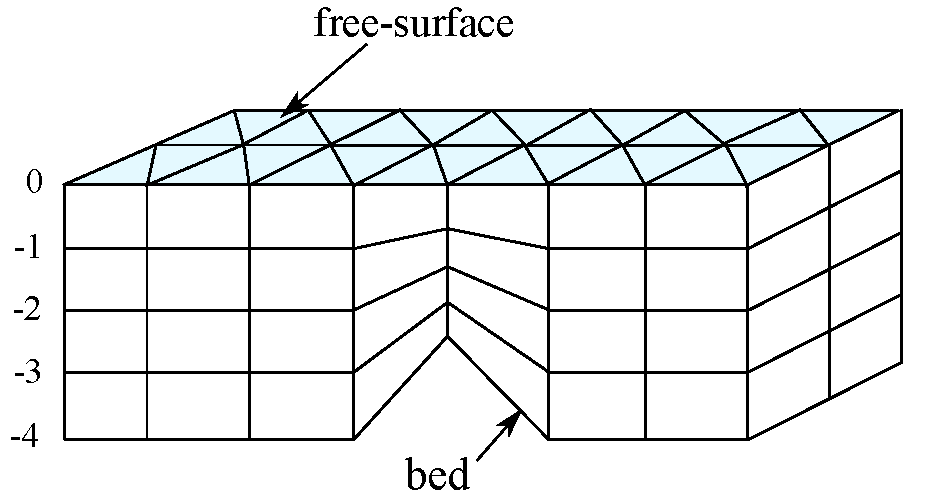
\includegraphics[scale=0.5]{graphics/classical_mesh.pdf}%
\caption{3-D mesh built from a 2-D mesh with a constant proportionality coefficient per plane.}%
\label{maillage 3D 1}%
\end{figure}

\nomenclature[D_z_ip]{$z_{ip}$}{$z$ component of node $i$ in plane $p$ \dotfill (m)}
\nomenclature[D_z*]{$z^*$}{$z$ component in the transformed domain \dotfill (-)}
\nomenclature[D_Delta_z]{$\Delta z$}{Height of a layer in the mesh;
can also be defined as $\partial z/\partial z^*$ \dotfill (m)}
\nomenclature[D_delta_t]{$\delta t$}{Time step \dotfill (s)}

\section{\label{maillage 3D}Building the three-dimensional mesh}

To build the three-dimensional domain with prisms, it is possible to build the
triangulation of the two-dimensional domain, then to repeat it along the
vertical in superimposed layers (called \textquotedblleft
planes\textquotedblright). These \textquotedblleft planes\textquotedblright%
\ are in fact surfaces with variable elevations. The only condition is that
the elevation of the points belonging to a vertical line should increase from the
bed to the free surface. Several simple formulae guarantee this condition,
as in the following four methods.

\subsection{\label{maillage 3D methode 1}Method 1: planes evenly spaced
along the vertical}

This first option, the most classic, consists of starting with the coordinate
nodes $(x,y)$ of the 2D mesh, then defining the elevation for each point of
the 3D mesh with coordinates $(x,y,z)$, according to the formula:%
\begin{equation}
z(x,y,ip)=b\left(  x,y\right)  +\dfrac{ip-1}{np-1}\left(  \eta\left(
x,y\right)  -b\left(  x,y\right)  \right)
\end{equation}
$b$ always being the bed elevation, $\eta$ the free surface elevation
and $ip$ is the rank of the plane under consideration (planes range from $1$
to $np$ if we go from the bed to the free surface). This is the simplest
method based on the sigma transformation (see the section \ref{sec:ALE}.
In this case the vertical coordinate $z^{\ast}$ of each plane in the
transformed mesh is simply $(ip-1)/(np-1)$. The figure \ref{maillage 3D 1}
is a representation of such a mesh.

\subsection{\label{maillage 3D methode 2}Method 2: data of a function
$\theta$ constant for each plane}

The coordinate $z^{\ast}$ of plane $ip$ in the transformed mesh is no longer
$(ip-1)/(np-1)$ but a given number $\theta_{ip}$ such that $0\leq
\theta_{ip}\leq1$ and, for intermediary planes, $\theta_{ip-1}<\theta
_{ip}<\theta_{ip+1}$. We now have:

\begin{equation}
z(x,y,ip)=b\left(  x,y\right)  +\theta_{ip}\left(  \eta\left(
x,y\right)  -b\left(  x,y\right)  \right)
\end{equation}

The figure \ref{maillage 3D 2} shows an example of a 3D mesh built with the
following values:
$\theta_{1}=0,\,\theta_{2}=1/6,\,\theta_{3}=1/3,\,\theta_{4}=2/3,\,\theta_{5}=1$, where the planes are numbered
from the bed to the free-surface. The choice of values of
$\theta_{ip}$ is free, the only constraints being a value of $0$ for the
bed ($ip=1$), a value of 1 for the free surface ($ip=np$) and a series of
intermediate values in a strictly increasing order.

\begin{figure}[tbh]
\centering
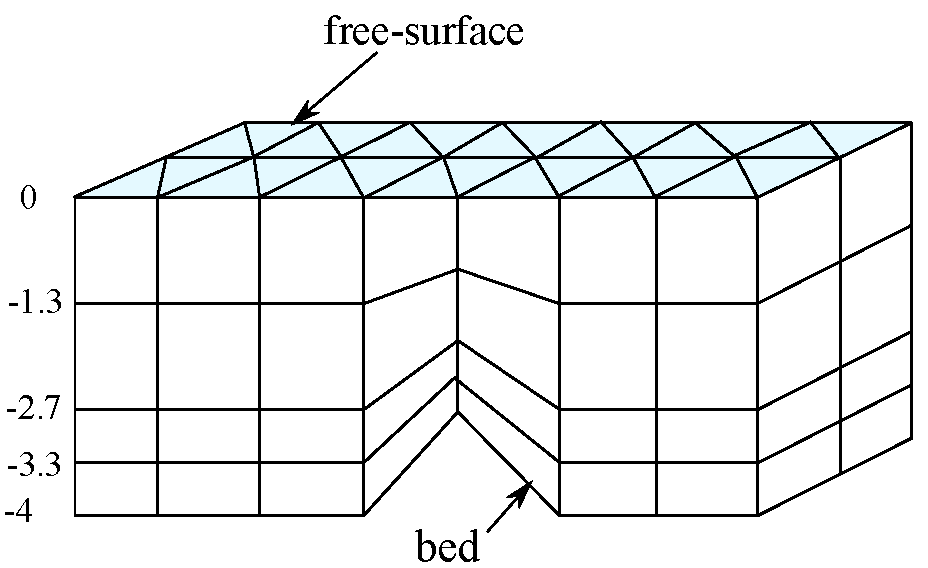
\includegraphics[scale=0.5]{graphics/mesh_theta.pdf}
\caption{Mesh built with a constant proportionality coefficient per plane.}%
\label{maillage 3D 2}
\end{figure}

\subsection{\label{maillage 3D methode 3}Method 3: double sigma transform}

Here we prescribe a constant elevation for one plane, then the planes between
the bed and this plane are evenly spaced, and the same is done between this
plane and the free surface.

\subsection{\label{maillage 3D methode 4}Method 4: horizontal planes}

In order to better represent the temperature stratification zones (thermoclines),
it is sometimes worth imposing a certain number of intermediate
planes to be horizontal. In this case, it is
possible to indicate the desired elevation for each plane, which will be
denoted by $z_{ip}$. This elevation is not always reachable because it can
be located below the bed or above the free surface. In this case, the
elevation of the point of the plane $ip$ will be maintained slightly above the
bed, or slightly below the free-surface. This can be done with the help of a
\textquotedblleft MinMod\textquotedblright\ limiter through the formula:%
\begin{equation}
z=\min\left\{  \max\left[  b(x,y)+\dfrac{ip-1}{np-1}d_{\min},z_{ip}\right]
,\eta(x,y,t)-\dfrac{np-ip}{np-1}d_{\min}\right\}
\end{equation}
where $d_{min}$ is an imposed minimum distance. We impose that plane 1 (the
bed) is at a minimum distance $d_{\min}$ from the free surface, and that
the plane $np$ (the free surface) is at a minimum distance $d_{min}$ from the bed.
The figure \ref{maillage 3D 3} shows an example of a 3D mesh built with this
method and the following prescribed elevations $z_{ip}$: $z_{1}=-4 m,\,z_{2}=-3 m,\,z_{3}%
=-2 m,\,z_{4}=-1 m,\,z_{5}=0 m$.%

\begin{figure}[tbh]%
\centering
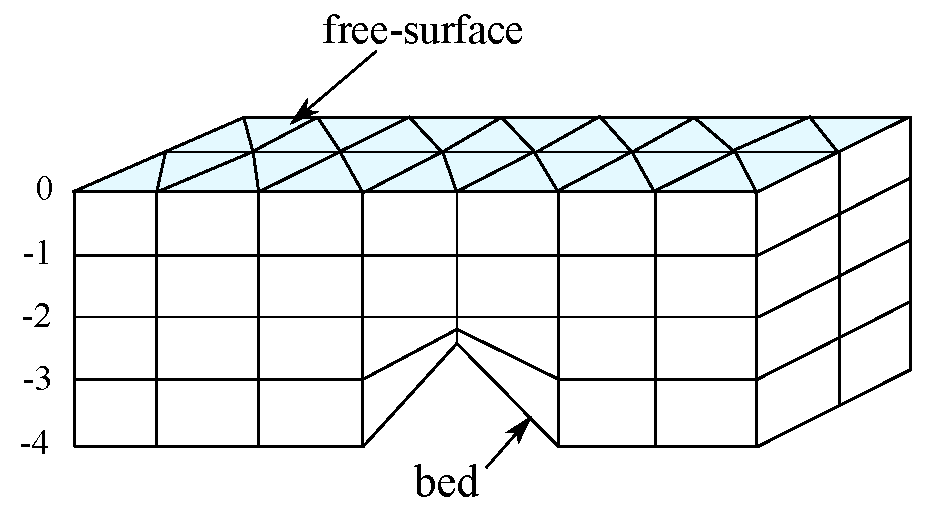
\includegraphics[scale=0.5]{graphics/mesh_horizontal_plane.pdf}
\caption{Example of a 3D mesh with a prescribed horizontal plane at $z=-2m$.}
\label{maillage 3D 3}%
\end{figure}

In conformity with the earlier formula, when the bed rises to the level of
plane number 2 normally situated at elevation $-$3 m, this plane number 2 then
adopts the form of the bed, at a distance $d_{min}/4$.

\begin{CommentBlock}{Comment by J.-M. Hervouet}
The advantage of this distribution is the elimination of truncation errors in
the calculation of buoyancy terms. These errors can generate unacceptable
instability when these terms are dominant. Actually, when the planes are not
horizontal, it is impossible to correctly represent a function $f$ that only
depends on $z$. Now, the density of the fluid should tend to this type of
function corresponding to a position of equilibrium without horizontal
pressure gradients.
With this method, non-horizontal mesh planes are inevitable, but only at a
distance less than $d_{min}$ from the bed or from the surface. In these
zones with quasi-zero volume, it is suggested that the forces arising from the
parasitic horizontal pressure gradients (called hydrostatic inconsistencies)
be cancelled by the intermediary of a filter which acts in places where the
prisms are, such that a node of the lower base (number 1, 2 or 3) has an
elevation higher than a node of the upper base (number 4, 5 or 6). This filter
also cancels the different diffusion coefficients on these elements.
\end{CommentBlock}

\section{\label{transformation sigma}Sigma transformation of the 3D mesh}

As the free surface evolves with time, the elevations $z$ of the 3D mesh vary
from one time step to another. However,
it is possible to change referentials so as to fix the mesh
during a time step. As we have already seen in the section \ref{sec:ALE}, this can
be particularly interesting in the advection step, which has a definite
influence on the evolution of the free surface. The change of variables
adopted in TELEMAC-3D is the sigma transformation, which consists in passing from the
coordinate $z$ to the coordinate $z^{\ast}$, the latter being independent of time.
For the classical sigma transformation, we recall the formula used:%
\begin{equation}
z^{\ast}=\dfrac{z-b}{\eta-b}%
\end{equation}

When a plane has a prescribed constant elevation, a double sigma transform is
preferred, with a function $z^{\ast}$ varying between $-$1 and +1.\ If
$z_{prescribed}$ is the required constant elevation, we have below the fixed plane:
\begin{equation}
z^{\ast}=\dfrac{z-z_{prescribed}}{z_{prescribed}-b}%
\end{equation}
and above:%
\begin{equation}
z^{\ast}=\dfrac{z-z_{prescribed}}{\eta-z_{prescribed}}%
\end{equation}

For a generalized sigma transform, it is convenient to use the following
function $z^{\ast}$ between planes $ip$ and $ip+1$:%
\begin{equation}
z^{\ast}=ip-1+\dfrac{z-z_{ip}}{z_{ip+1}-z_{ip}}%
\end{equation}
where $z_{ip}$ is the elevation of plane $ip$, and$\ z_{ip+1}$ the elevation
of plane $ip+1$. This function $z^{\ast}$ now varies between 0 and $np-1$.
The definition of $z^{\ast}$ is thus univocal over the entire vertical.

\begin{CommentBlock}{Remark:}
These forms of transformation are only necessary when dealing with the full 3D
mesh, \textit{e.g.} during an advection step with the method of characteristics.
For local computations within a single finite element, a local definition is simpler, which reads:
\begin{equation}
z^{\ast}=\dfrac{z-z_{ip}}{z_{ip+1}-z_{ip}}
\end{equation}
\textit{i.e.} we have a classic sigma transformation between two planes.
\end{CommentBlock}

It is interesting to notice that the four methods given above to build the mesh
belong to two different families:
\begin{itemize}
\item the first two are such that $\partial z/\partial z^{\ast}=h$, they thus rely on the classic sigma transformation
\item for the last two, which correspond to generalized sigma transformations:
\begin{equation}
\dfrac{\partial z}{\partial z^{\ast}}=z_{ip+1}-z_{ip}=\Delta z
\end{equation}
\textit{i.e.} the width between two planes, denoted by $\Delta z$. It is only
piecewise constant vertically.
\end{itemize}


\section{\label{equations de transport}Solving transport equations in 3D
\index{advection}%
}

\begin{WarningBlock}{Section under construction}
This section directly comes from the last TELEMAC-3D release notes and has not been
reshaped yet. It contains some explanations regarding the advection schemes but
no general description of the schemes themselves. The notations used in this
section are also the ones from the last release notes.
\end{WarningBlock}

Here we assume that the general problem of advection schemes is known, and we
shall not fully explain the principle of the different techniques. We just
give details on the 3D theory and implementation in specific cases, namely the
method of characteristics, distributive schemes, and the treatment of the
settling velocity.

\subsection{\label{methode des caracteristiques}Method of characteristics%
\index{characteristic curves}%
}

A lot of litterature can be found on the method of characteristics, but in the
case of advection it merely consists in computing pathlines of the flow,
called characteristics (actually trajectories or streamlines if the velocity
is considered constant in time). In the absence of terms other than advection,
the advected variables are constant on the characteristics, and are thus taken
at the previous time step at what is called the foot of the characteristic,
namely the place where was a particule of water that is now on a given point
of the mesh, at the previous time step. \ Basically the method of
characteristics is thus a computation of trajectory followed by an
interpolation. We shall not here describe the navigation in the mesh and how
it works in parallel, but just deal with the specific 3D aspects, the fact
that the advection in TELEMAC-3D is done in a transformed mesh to account for
relocalisation. The theory behind the vertical displacements in the method of
characteristics in 3D is as a matter of fact very tricky and we give hereafter
some explanations. The first thing to understand is that the advection
equation is solved in a transformed mesh with horizontal planes. The sigma
transformation is used to take into account the movement of the mesh.\ As a
matter of fact the physical values at a point in the mesh will change due to
advection terms (velocity of flow) but also due to the movement of the mesh.
It is shown in reference \cite{hervouet007}\ page 21, equation 2.90\ that this can
be simply taken into account by an advection in the transformed mesh. One
would thus expect that the vertical displacements when computing the
characteristics pathlines are of the form:%
\begin{equation}
\Delta z^{\ast}=w^{\ast}\delta t
\end{equation}
using the transformed coordinates and the transformed velocities, but we find
in the implementation the following form:
\begin{equation}
\Delta z^{\ast}=w~\dfrac{ZSTAR(IET+1)-ZSTAR(IET)}{\Delta z}~\delta t
\end{equation}
where $\Delta z$ is the local real width of the given layer between two planes
and $ZSTAR$ is the transformed elevation of planes (here $IET+1$ and $IET$) in
the transformed mesh.

The second thing to understand is then that the velocity $w$ provided by
TELEMAC-3D to the subroutine CHARAC is in fact $w^{\ast}\Delta z$. This
quantity is provided by the subroutine TRIDW2 and has the dimension of a
velocity, it is linked to the real vertical velocity by the formula:%
\begin{equation}
w=\dfrac{\partial z}{\partial t}+u\dfrac{\partial z}{\partial x}+v\dfrac{\partial
z}{\partial y}+w^{\ast}\dfrac{\partial z}{\partial z^{\ast}}%
\end{equation}
where $\partial z/\partial z^{\ast}$ is $\Delta z$ when we apply a
sigma transformation that changes a layer of width $\Delta z$ into a layer of
width 1. Our vertical displacements are thus in reality:%
\begin{equation}
\Delta z^{\ast}=w^{\ast}\dfrac{\partial z}{\partial z^{\ast}}~\dfrac
{ZSTAR(IET+1)-ZSTAR(IET)}{\Delta z}~\delta t
\end{equation}
and $(ZSTAR(IET+1)-ZSTAR(IET))/\Delta z$ is here to give the value
$\partial z^{\ast}/\partial z$ that retrieves the wanted formula
$\Delta z^{\ast}=w^{\ast}\delta t$. At this level we understand that the
values of ZSTAR must correspond to a sigma transformation that changes a layer
$\Delta z$ into a layer of width 1. A solution would be for example that we
have ZSTAR(IET)=IET. This would be simple but this is not exactly what is done.

The third thing to understand:

Actually we are free to apply any correction factor in the vertical
displacements if they are taken into account also in the values of ZSTAR. In
other words we can multiply the coordinates in a layer by any constant without
changing the result. The interest is then that the correction factor
$(ZSTAR(IET+1)-ZSTAR(IET))/\Delta z$ could be a constant independent of
the layer.\ Then the displacements would keep their meaning all over the mesh.
Otherwise we would have to stop at every plane, and recompute a new
displacement compatible with the new metrics (this is done with the
generalised sigma transformation). The denominator being the real width, our
correction factor will be constant if the values of ZSTAR are proportional to
the real z coordinates, for example if they are the values of the array ZSTAR
used for building the mesh, i.e. a sigma transformation giving the whole 3D
mesh a width of 1. For a classical sigma transformation, we have then:%
\begin{equation}
ZSTAR(IET)=\dfrac{IET-1}{NPLAN-1}%
\end{equation}
where NPLAN is the number of planes. The final formula thus mixes two
different sigma transformations, one for computing $w^{\ast}$, one for the
local metrics while navigating in the transformed mesh, and this is not a mistake.

\subsection{\label{schema murd en dimension 3}MURD scheme in three dimensions%
\index{MURD scheme}%
}

The MURD scheme of Janin \cite{janin95}, which signifies \textquotedblleft
Multidimensional Upwind Residual Distribution\textquotedblright, is an
adaptation to prisms of the N and PSI schemes that we have just described for
the triangular meshes. We shall look successively at the two variants: N and PSI.

\subsubsection{N-type MURD scheme}

We work with the transformed fixed mesh and we want to guarantee the global
conservation of the function $f$ by showing that one has:%

\begin{equation}
\int\nolimits_{\Omega^{\ast}}\,\Delta z^{n+1}\dfrac{(f^{n+1}-f^{n})}{\delta t}~
d\Omega^{\ast}+\int\nolimits_{\Omega^{\ast}}\Delta z\vec{u}^{\ast}
\cdot\Grad f^{n}~d\Omega^{\ast}=0
\end{equation}
based on our local equations. We recall that $\vec{u}^{\ast}$ is
made up of the components ($u,v,w^{\ast}$).

The first term is initially written as:%

\begin{equation}
\int\nolimits_{\Omega^{\ast}}\Delta z^{n+1}\dfrac{(f^{n+1}-f^{n})}{\delta
t}~d\Omega^{\ast}=\sum\limits_{ip=1}^{np}\dfrac{(f_{ip}^{n+1}-f_{ip}^{n}%
)}{\delta t}\int\nolimits_{\Omega^{\ast}}\Psi_{ip}^{\ast}\Delta
z^{n+1}~d\Omega^{\ast}
\end{equation}
We later denote:
\begin{equation}
\int\nolimits_{\Omega^{\ast}}\Psi_{ip}^{\ast}\,\Delta z^{n+1}~d\Omega^{\ast
}=S_{ip}%
\end{equation}
to obtain
$\sum\nolimits_{ip=1}^{np}(f_{ip}^{n+1}-f_{ip}^{n})S_{ip}/\delta t$,
the first term of the equation of a point $ip$.
For the second term, $\int\nolimits_{\Omega^{\ast}}\Delta z\vec{u}
\cdot\Grad f^{n}~d\Omega^{\ast}$, we
shall calculate it element by element, and for each element share the
contributions over the points it is made up of. The sum of all our equations
will again give us the global equation desired.

By limiting ourselves to a prism $P^{\ast}$ of the transformed mesh, we shall
thus try to calculate:%

\begin{equation}
\Phi_{P}=\int\nolimits_{P^{\ast}}\Delta z\vec{u}\cdot\Grad(f)~dP^{\ast}
\end{equation}
by trying to put it into the form:
\begin{equation}
\Phi_{P}=\sum\limits_{i=1}^{6}\sum\limits_{j=1}^{6}\lambda_{ij}(f_{i}^{n}-f_{j}^{n})
\end{equation}
with the coefficients $\lambda_{ij}$ positive or zero, as we did for the N
scheme. By decomposing $f$, we already know that:

\begin{equation}
\Phi_{P}=\sum\limits_{i=1}^{6}f_{i}^{n}\int\nolimits_{P^{\ast}}\Delta
z\vec{u}\cdot\Grad\Psi_{i}~dP^{\ast}%
\end{equation}

Now the terms:%
\begin{equation}
\int\nolimits_{P^{\ast}}\Delta z\vec{u}\cdot\Grad\Psi_{i}~dP^{\ast}%
\end{equation}
can be decomposed in horizontal or vertical gradients in the form $a_{i}%
+b_{i}$ with:
\begin{equation}
a_{i}=\int\nolimits_{P^{\ast}}\Delta z u\dfrac{\partial\Psi_{i}}{\partial
x}~dP^{\ast}+\int\nolimits_{P^{\ast}}\Delta z v\dfrac{\partial\Psi_{i}%
}{\partial y}~dP^{\ast}%
\end{equation}
and:%
\begin{equation}
b_{i}=\int\nolimits_{P^{\ast}}\Delta zw^{\ast}\dfrac{\partial\Psi_{i}}{\partial
z^{\ast}}\,dP^{\ast}%
\end{equation}

As we did in Section \ref{wstarmoyen}, we now decompose the bases $\Psi
_{i}(x,y,z^{\ast})$ of the prism into the product $\Psi_{i}^{h}(x,y)\Psi
_{i}^{v}(z^{\ast})$, which gives:%

\begin{equation}
a_{i}=\dfrac{\partial\Psi_{i}^{h}}{\partial x}\int\nolimits_{P^{\ast}}\Delta
z u\Psi_{i}^{v}\,dP^{\ast}+\dfrac{\partial\Psi_{i}^{h}}{\partial y}%
\int\nolimits_{P^{\ast}}\Delta z v\Psi_{i}^{v}\,dP^{\ast}%
\end{equation}
and:%

\begin{equation}
b_{i}=\dfrac{\partial\Psi_{i}^{v}}{\partial z^{\ast}}\int\nolimits_{P^{\ast}%
}\Delta zw^{\ast}\Psi_{i}^{h}\,dP^{\ast}%
\end{equation}

The properties of the bases $\Psi_{i}^{h}(x,y)$ and $\Psi_{i}^{v}(z^{\ast})$
then give us a group of properties for coefficients $a_{i}$ and $b_{i}$:

\begin{itemize}
\item $a_{1}+a_{2}+a_{3}=0$ inferred by $\Psi_{1}^{h}+\Psi_{2}^{h}+\Psi
_{3}^{h}=1$

\item $a_{4}+a_{5}+a_{6}=0$ inferred by $\Psi_{4}^{h}+\Psi_{5}^{h}+\Psi
_{5}^{h}=1$

\item $b_{1}+b_{4}=0$ inferred by $\Psi_{1}^{v}+\Psi_{4}^{v}=1$

\item $b_{2}+b_{5}=0$ inferred by $\Psi_{2}^{v}+\Psi_{5}^{v}=1$

\item $b_{3}+b_{6}=0$ inferred by $\Psi_{3}^{v}+\Psi_{6}^{v}=1$
\end{itemize}

Here, we have again used the local numbering of the points in a prism.

Based on the N scheme, which is built on triangles, a first set of
coefficients $\lambda_{ij}$ could be the following:

\begin{itemize}
\item $\lambda_{ij}=\max(\min(a_{i},-a_{j}),0)$ for the points $i$ and $j$ of
the lower triangle of the prism, or for those of the upper triangle.

\item $\lambda_{i\,i+3}=\max(b_{i},0)$ for the points $i$ of the lower triangle.

\item $\lambda_{i+3\,i}=\max(b_{i+3},0)$ for the points $i$ of the upper triangle.

\item $\lambda_{ij}=0$ for the other terms (which are \textquotedblleft
crossed\textquotedblright\ terms, linking the points which are neither at the
same level, nor on the same vertical line).
\end{itemize}

We already possess all the good properties to construct an N-type scheme (all
the coefficients are positive or zero). However, one could obtain a less
diffusive scheme by transforming the sums of horizontal and vertical fluxes
into crossed fluxes, which can be done by noticing that for a set of three
coefficients $\lambda_{ij}$, $\lambda_{jk}$ and $\lambda_{ik}$, one does not
change the value of $\Phi_{P}$ by carrying out the following series of operations:

\begin{itemize}
\item $\lambda_{ik}=\lambda_{ik}+\min(\lambda_{ij},\lambda_{jk})$

\item $\lambda_{ij}=\lambda_{ij}-\min(\lambda_{ij},\lambda_{jk})$

\item $\lambda_{jk}=\lambda_{jk}-\min(\lambda_{ij},\lambda_{jk})$
\end{itemize}

One in fact observes that the coefficients of $f_{i}^{n}$, $f_{j}^{n}$ and
$f_{k}^{n}$ remain unchanged. We now have a supplementary property, which is
that if a coefficient $\lambda_{ij}$ is strictly positive, then all the
coefficients $\lambda_{jk}$ are zero.

We shall choose, as in two dimensions, the distribution coefficients
$\beta_{i}$ as:%

\begin{equation}
\beta_{i}\Phi_{P}=\sum\limits_{j=1}^{6}\lambda_{ij}(f_{i}^{n}-f_{j}^{n})
\end{equation}
in order to obtain an N-type scheme. Here again, we find a stability criterion
in order to ensure the monotonicity of the scheme:%

\begin{equation}
\delta t\leq\dfrac{S_{i}}{\sum\limits_{\text{neighbouring\thinspace\thinspace
prisms}}\lambda_{ij}}%
\end{equation}


\subsubsection{PSI-type MURD scheme}

Based on our newly found N-type scheme, we need to construct the PSI-type
scheme that will also guarantee that the distribution coefficients fall
between 0 and 1. To do this, in the calculation of $\Phi_{P}$ we need to
separate the positive and negative contributions:%

\begin{equation}
\Phi_{P}=\Phi_{P}^{+}-\Phi_{P}^{-}=\sum\limits_{j=1}^{6}\lambda_{ij}\max
(f_{i}^{n}-f_{j}^{n},0)-\sum\limits_{j=1}^{6}\lambda_{ij}\max(f_{j}^{n}%
-f_{i}^{n},0)
\end{equation}


By comparing $\Phi_{P}^{+}$ and $\Phi_{P}^{-}$, one can modify the scheme N coefficients:

If $\Phi_{P}^{+}\geq\Phi_{P}^{-}$:

\qquad If $f_{j}^{n}\geq f_{i}^{n}$, then $\lambda_{ij}$ is cancelled,

\qquad otherwise $\lambda_{ij}$ is replaced by $\lambda_{ij}\Phi_{P}/\Phi_{P}^{+}$.

If $\Phi_{P}^{+}\leq\Phi_{P}^{-}$:

\qquad If $f_{j}^{n}\geq f_{i}^{n}$, then $\lambda_{ij}$ is replaced by
$-\lambda_{ij}\Phi_{P}/\Phi_{P}^{-}$,

\qquad otherwise $\lambda_{ij}$ is cancelled.

The following is an explanation of these manipulations. In the case where the
positive contributions are the most important, we multiply them by $\Phi_{P}/\Phi_{P}^{+}$
and we cancel the negative contributions. What was $\Phi_{P}^{-}$ is thus cancelled,
what was $\Phi_{P}^{+}$ becomes $\Phi _{P}^{+}\Phi_{P}/\Phi_{P}^{+}=\Phi_{P}$. The final expression for
$\Phi_{P}$ remains unchanged. The case $\Phi_{P}^{+}\leq\Phi_{P}^{-}$ can
easily be deduced.

Following this modification of the coefficients $\lambda_{ij}$, all the terms
$\lambda_{ij}(f_{i}^{n}-f_{j}^{n})$ are positive and all the terms $\beta_{i}$
fall between 0 and 1. Actually:%

\begin{equation}
\beta_{i}=\dfrac{\sum\limits_{j=1}^{6}\lambda_{ij}(f_{i}^{n}-f_{j}^{n})}%
{\Phi_{P}}=\dfrac{\sum\limits_{j=1}^{6}\lambda_{ij}(f_{i}^{n}-f_{j}^{n})}%
{\sum\limits_{l=1}^{6}\sum\limits_{j=1}^{6}\lambda_{ij}(f_{l}^{n}-f_{j}^{n})}%
\end{equation}


All the terms of the summations are positive and the numerator is smaller than
the denominator.

\paragraph{\label{murdconservation}Remarks on mass conservation with the
MURD scheme}

The MURD scheme is perfectly compatible with the proof of scalar mass
conservation set out in Section \ref{masse traceur} and with the continuity
step described in Section \ref{wstarmoyen}. We have in fact said in this
section that:%

\begin{equation}
\Delta zw^{\ast}=\sum\limits_{j=1}^{npoin2}\left[  \Delta zw^{\ast}(z^{\ast
})\right]  _{j}\Psi_{i}^{h}(x,y)
\end{equation}
and $\Delta zw^{\ast}$ is necessary here to calculate the coefficients:%

\begin{equation}
b_{i}=\dfrac{\partial\Psi_{i}^{v}}{\partial z^{\ast}}\int\nolimits_{P^{\ast}%
}\Delta zw^{\ast}\Psi_{i}^{h}\,dP^{\ast}%
\end{equation}


We thus find that:%

\begin{equation}
b_{i}=\sum\limits_{j=1}^{npoin2}\int\nolimits_{\Omega_{2D}}\Psi_{i}^{h}%
\Psi_{j}^{h}\,d\Omega_{2D}\,\,\left\{  \dfrac{\partial\Psi_{i}^{v}}{\partial
z^{\ast}}\int\nolimits_{z_{ip}^{\ast}}^{z_{ip+1}^{\ast}}\left[  \Delta
zw^{\ast}\right]  _{j}\,dz^{\ast}\right\}
\end{equation}


We see that the term in brackets is (ignoring the sign):%

\begin{equation}
\dfrac{1}{(z_{ip}^{\ast}-z_{ip+1}^{\ast})}\int\nolimits_{z_{ip}^{\ast}%
}^{z_{ip+1}^{\ast}}\left[  \Delta zw^{\ast}(z^{\ast})\right]  _{j}~dz^{\ast}%
\end{equation}
which we have denoted $\overline{\left(  \Delta zw^{\ast}\right)}_{ip+1/2}^{j}$.
These terms are produced to resolve the continuity equation.
If mass lumping has been used when computing $\overline{\left(\Delta zw^{\ast}\right)}_{ip+1/2}^{j}$
(see the note at the end of the section \ref{wstarmoyen}), then the coefficients $b_{i}$ must be computed in a
compatible way, which is:%

\begin{equation}
b_{i}=\int\nolimits_{\Omega_{2D}}\Psi_{i}^{h}\,d\Omega_{2D}\,\,\left\{
\dfrac{\partial\Psi_{i}^{v}}{\partial z^{\ast}}\int\nolimits_{z_{ip}^{\ast}%
}^{z_{ip+1}^{\ast}}\left[  \Delta zw^{\ast}\right]  _{i}\,dz^{\ast}\right\}
\end{equation}


%\subsection{A finite volume advection solver}
%
%The main idea is to design an advection solver close to what is done with the
%distributive scheme, i.e. with a splitting of time to ensure the CFL
%condition, with the only modification that the fluxes taken into account are
%not the finite element fluxes, but rather the finite volume point to point
%fluxes which are currently built for the Delwaq interface and for the
%treatment of negative depths in 3D. In 3D and with distributive schemes (full
%explanations on distributive schemes are given in reference \cite{hervouet007}\ from
%page 183 on) we just recall here that we end up in a discretization of
%advection equation in the form:%
%
%\begin{equation}
%S_{i}(\dfrac{C_{i}^{n+1}-C_{i}^{n}}{\delta t})=-\beta_{i}\Phi_{T}%
%\end{equation}
%
%
%Where $S_{i}$ is the integral of the test function of point $i$, $\beta_{i}$
%is a distribution coefficient, $\delta t$ the time step, $C_{i}^{n+1}$the
%value of function $C$ at point $i$ after advection, $C_{i}^{n}$ the value of
%function $C$ at point $i$ before advection. $\Phi_{T}$ actually represents
%$S_{i}(\vec{u}.\Grad(C))$ where $\vec{u}
%$ is the advecting field. The only thing to know here is that $\beta_{i}%
%\Phi_{T}$ is eventually put in the form:%
%
%\begin{equation}
%\beta_{i}\Phi_{T}=\sum\limits_{j}\lambda_{ij}(C_{i}-C_{j})
%\end{equation}
%where the coefficients $\lambda_{ii}$ are zero and all coefficients
%$\lambda_{ij}$ are positive or zero. The sum is done on all the neighbouring
%points of point $i$, i.e. all the points that belong to an element containing
%$i$.
%
%The final value of function $C$ at point $i$ is thus:%
%
%\begin{equation}
%C_{i}^{n+1}=C_{i}^{n}\left(  1-\sum\limits_{j}\lambda_{ij}\dfrac{\delta
%t}{S_{i}}\right)  +\sum\limits_{j}\dfrac{\delta t}{S_{i}}\lambda_{ij}C_{j}^{n}
%\label{finalvalue}%
%\end{equation}
%
%
%Classically, it is said then that the monotonicity criterion consists in
%ensuring that all the coefficients of $f_{i}^{n}$ and $f_{j}^{n}$ be positive,
%which yields, given the fact that all $\lambda_{ij}$ are positive or zero:%
%
%\begin{equation}
%\delta t\leq\dfrac{S_{i}}{\sum\limits_{j}\lambda_{ij}}%
%\end{equation}
%
%
%In finite volumes with fluxes between points, the corresponding equation would be:%
%
%\begin{equation}
%C_{i}^{n+1}=\left(  1-\dfrac{\delta t}{S_{i}}\sum\limits_{j}\max(\Phi
%_{ij},0)\right)  C_{i}^{n}+\sum\limits_{j\text{ }}\dfrac{\delta t}{S_{i}}%
%\max(\Phi_{ij},0)C_{j}^{n}%
%\end{equation}
%
%
%assuming that we start from element by element fluxes in the form:%
%
%\begin{equation}
%\Phi_{i}^{el}=\int\nolimits_{\Omega}\vec{u}.\Grad%
%(\Psi_{i})~d\Omega
%\end{equation}
%
%
%this explains the difference of signs with what was done in 2D where we start
%from fluxes in the form:%
%
%\begin{equation}
%\Phi_{i}^{el}=-\int\nolimits_{\Omega2d}h\vec{u}%
%.\Grad(\Psi_{i})~d(\Omega2d)
%\end{equation}
%
%
%which are fluxes leaving points. This leads us to the following CFL\ condition:%
%
%\begin{equation}
%\delta t\leq\dfrac{S_{i}}{\sum\limits_{j}\max(\Phi_{ij},0)}%
%\end{equation}
%
%
%Implementation should be the same provided that we change everywhere
%$\lambda_{ij}$ by max$(\Phi_{ij},0)$.
%
%In fact, the distributive scheme implementation in subroutine murd3d.f in
%Telemac only uses $\sum\limits_{j}\lambda_{ij}(C_{j}^{n}-C_{i}^{n})$ which is
%array $TRA02$ and $-\sum\limits_{j}\lambda_{ij}$ which is put in array $DB$. A
%finite volume upwind scheme can then be easily implemented if we take:%
%
%\begin{equation}
%DB=-\sum\limits_{j}\max(\Phi_{ij},0)
%\end{equation}
%
%
%and%
%
%\begin{equation}
%TRA02=\sum\limits_{j}\max(\Phi_{ij},0)(C_{j}^{n}-C_{i}^{n})
%\end{equation}
%
%
%Starting from the coefficients $\Phi_{i}^{el}$ (six per element), the point to
%point coefficients $\Phi_{ij}$ are obtained as is done in the interface to
%Delwaq, i.e.:
%
%1) assembling element by element fluxes on points: horizontal fluxes will be a
%sum of two contributions (from the upper and lower layer, except on the bed
%and the free surface).
%
%2) changing the horizontal fluxes of points 1, 2, and 3 in the prism into
%point to point fluxes.\
%
%Points 1 and 2 are done in a subroutine called fluxvfleo\_3d, which calls the
%2D subroutine fluxvfleo.f
%
%3) cancelling all crossed fluxes (between points 1 and 5, 1 and 6, 2 and 4, 2
%and 6, 3 and 4, 3 and 5)
%
%4) finding the vertical fluxes that solve the continuity equation. Comparing
%what is done in subroutine tridw2.f and in subroutine tel4del.f, we find that
%the vertical fluxes are such that:%
%
%\begin{equation}
%\Phi_{ij}=-\Delta z~w^{\ast}%
%%TCIMACRO{\dint \nolimits_{\Omega2d}}%
%%BeginExpansion
%{\displaystyle\int\nolimits_{\Omega2d}}
%%EndExpansion
%\Psi_{k}d(\Omega2d)
%\end{equation}
%
%
%where $\Phi_{ij}$ is the vertical flux between to points $i$ and $j$ located
%in the same prism, on the vertical of the 2D point $k$. On a total of 15
%possible fluxes in the prism, we thus retain 9 non-zero terms, which is
%exactly what is done also with the N-scheme, with the same vertical fluxes.
%Both schemes are actually very close, though different, and it was very easy
%to add the new finite volume scheme as a variant of distributive scheme, in
%subroutine murd3d.f.

\subsection{The case of settling velocity}

We explain here how is done the new advection matrix for the treatment of the
settling velocity $w_{c}$. The treatment described here corresponds to the
keyword ADVECTION-DIFFUSION SCHEME WITH SETTLING VELOCITY = 0, i.e. the
settling velocity is taken into account in a fully implicit way in the
diffusion step. The former treatment consisted of computing first a centered
advection term (call to MATRIX with formula 'MATFGR \ \ \ \ \ \ \ \ \ Z'), and
then upwinding (subroutine upwind, which merely adds a diffusion with a
coefficient $\Delta z~w_{c}/2$, where $\Delta z$\ is the local mesh
size on the vertical). Though this technique would give a perfectly implicit
upwind scheme in a regular one-dimensional mesh, it is more difficult to prove
stability and monotonicity in our 3-dimensional context, with $\Delta z $
depending on the layer and on the position in the underlying 2D mesh.

Our starting equation is in the continuum:%

\begin{equation}
\dfrac{\partial C}{\partial t}+\operatorname{div}(-\vec{w_{c}}C)=0
\end{equation}


As $w_{c}$ is considered positive (version 7.0 on...), we have added the sign
minus to recall that $\vec{w_{c}}$ is a vector pointing downwards.
The equation is solved in the fixed mesh taken at the end of the time step
(since this is also done with diffusion). It is important to start from an
equation written in a conservative form, because $\vec{w_{c}}$ may
be variable in space, and has no reason to be divergence free. Moreover it has
nothing to see with the ambient flow, which would have to be used to simplify
into a non conservative equation.

After discretising the derivative in time and variational formulation, our
equation gives for every point $i$:%

\begin{equation}%
%TCIMACRO{\dint \nolimits_{\Omega}}%
%BeginExpansion
{\displaystyle\int\nolimits_{\Omega}}
%EndExpansion
\Psi_{i}\dfrac{(C^{n+1}-C^{n})}{\delta t}~d\Omega+%
%TCIMACRO{\dint \nolimits_{\Omega}}%
%BeginExpansion
{\displaystyle\int\nolimits_{\Omega}}
%EndExpansion
\Psi_{i}\operatorname{div}(-\vec{w_{c}}C)~d\Omega=0
\end{equation}


Then we integrate by parts the divergence term:%

\begin{equation}%
%TCIMACRO{\dint \nolimits_{\Omega}}%
%BeginExpansion
{\displaystyle\int\nolimits_{\Omega}}
%EndExpansion
\Psi_{i}\dfrac{(C^{n+1}-C^{n})}{\delta t}~d\Omega-%
%TCIMACRO{\dint \nolimits_{\Gamma}}%
%BeginExpansion
{\displaystyle\int\nolimits_{\Gamma}}
%EndExpansion
\Psi_{i}C\vec{w_{c}}~.\vec{n}~d\Gamma+%
%TCIMACRO{\dint \nolimits_{\Omega}}%
%BeginExpansion
{\displaystyle\int\nolimits_{\Omega}}
%EndExpansion
\vec{w_{c}}C\Grad(\Psi_{i}%
)~d\Omega=0
\end{equation}


The boundary term is treated in the boundary conditions, it is on one side the
flux coming from the free surface (i.e. zero) and on the other side the
deposition on the bed. The deposition is discretised with an implicit
concentration, and with mass-lumping, i.e. with the approximation
${\displaystyle\int\nolimits_{\Gamma}}
\Psi_{i}C\vec{w_{c}}~.\vec{n}~d\Gamma\simeq C_{i}^{n+1}%
{\displaystyle\int\nolimits_{\Gamma}}
\Psi_{i}\vec{w_{c}}~.\vec{n}~d\Gamma$. If $w_{c}$ is
constant we see clearly that this term is $-w_{c}C_{i}^{n+1}
{\displaystyle\int\nolimits_{\Omega_{2d}}}
\Psi_{i}~d\Omega_{2d}$. $\Omega_{2d}$ refers to the 2D mesh and is horizontal.
${\displaystyle\int\nolimits_{\Omega_{2d}}}\Psi_{i}~d\Omega_{2d}$
is the area around point $i$ (equivalent to the finite
volume). This term is negative (seen from the suspension it is a loss of
sediment), this is why it is treated implicitly.

Now the matrix corresponding to the term ${\displaystyle\int\nolimits_{\Omega}}
\Psi_{i}\operatorname{div}(-\vec{w_{c}}C)~d\Omega=0$:

This term represents the internal fluxes that change the concentration of a
point (think that ${\int_{\Omega}}\Psi_{i}(C^{n+1}-C^{n})/\delta t~d\Omega$ is the variation of mass).
The matrix will be built element by element, so we restrict to a single prism.
The area associated to points is $SURFAC/3$, where $SURFAC$\ is the area of
the triangle formed by a projection on the horizontal of upper and lower sides
of the prism, or the corresponding triangle in the 2D mesh. Assembling all
$SURFAC/3$ of elements around a point gives ${\displaystyle\int
\nolimits_{\Omega_{2d}}}\Psi_{i}~d\Omega_{2d}$,
the integral of the 2D basis of this point.%

\begin{figure}[h]%
\centering
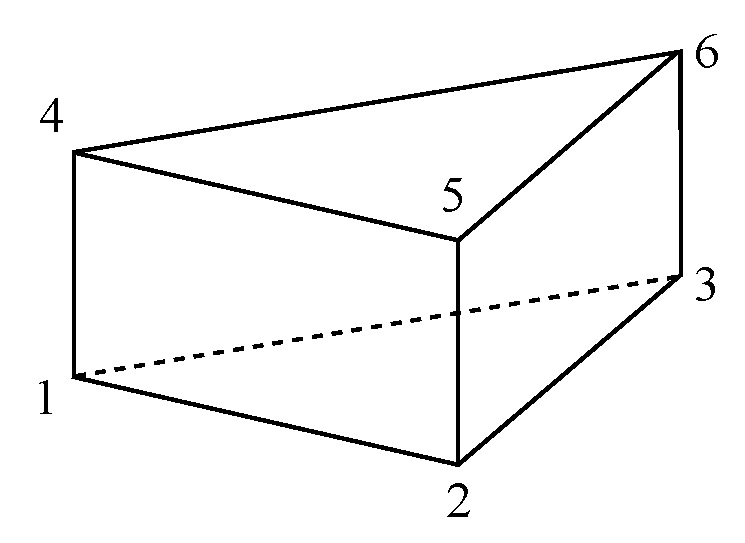
\includegraphics[scale=0.5]{graphics/prism_numbering.pdf}
\caption{Sketch of the prismatic element used in TELEMAC-3D and of the local numbering convention for the nodes.}
\label{schema prisme}%
\end{figure}

To have an upwind treatment of advection we decide that:
\begin{itemize}
\item point 4 looses a flux of $C^{n+1}(4)w_{c}(4)SURFAC/3$
\item point 5 looses a flux of $C^{n+1}(5)w_{c}(5)SURFAC/3$
\item point 6 looses a flux of $C^{n+1}(6)w_{c}(6)SURFAC/3$
\item point 1 receives from point 4 a flux of $C^{n+1}(4)w_{c}(4)SURFAC/3$
\item point 2 receives from point 5 a flux of $C^{n+1}(5)w_{c}(5)SURFAC/3$
\item point 3 receives from point 6 a flux of $C^{n+1}(6)w_{c}(6)SURFAC/3$
\end{itemize}
If we restrict to fluxes into the prism this is all what we see. Of course the
upper points also receive from the upper prism and the lower points give to a
lower prism, but if we restrict here to what we see in the prism there will be
no duplication, and only what receive the points at the free surface and what
give the points at the bed will be forgotten, and it is actually the
boundary terms which are treated elsewhere.

The six fluxes mentionned above result in 6 non zero terms of the element by
element matrix, namely:

$-w_{c}(4)SURFAC/3\qquad$(coefficient of point 4 in equation of point 1, which
is XM(ielem,3))

$-w_{c}(5)SURFAC/3\qquad$(coefficient of point 5 of equation of point 2, which
is XM(ielem,8))

$-w_{c}(6)SURFAC/3\qquad$(coefficient of point 6 of equation of point 3, which
is XM(ielem,12))

$w_{c}(4)SURFAC/3\qquad$(diagonal of 4, which is T(ielem,4))

$w_{c}(5)SURFAC/3\qquad$(diagonal of 5, which is T(ielem,5))

$w_{c}(6)SURFAC/3\qquad$(diagonal of 6, which is T(ielem,6))

This is what is done in subroutine mt15pp.f, then these terms may be assembled
to give the final matrix.

The process of points giving a quantity that is received by others is a proof
of mass-conservation. Note that the diagonals receive positive numbers and the
off-diagonal terms receive negative numbers. The matrix thus built is then a
M-matrix and this ensures the positivity. The matrix will remain always positive-definite.

It would be better to consider that the settling velocities are piece-wise
constant on the vertical, so that we do not consider the settling velocity of
upper points, but an average velocity on the way between upper points and
lower points.

%%%%%%%%%%%%%%%%%%%%%%%%%%%%%%%%%%%%%%%%%%%%%%%%%%%%%%%%%%%%%%%%%%%%%%%%%%%%%%%%%%%%%%%%
%%%%%%%%%%%%%%%%%%%%%%%%%%%%%%%%%%%%%%%%%%%%%%%%%%%%%%%%%%%%%%%%%%%%%%%%%%%%%%%%%%%%%%%%
%%%%%%%%%%%%%%%%%%%%%%%%%%%%%%%%%%%%%%%%%%%%%%%%%%%%%%%%%%%%%%%%%%%%%%%%%%%%%%%%%%%%%%%%
%%%%%%%%%%%%%%%%%%%%%%%%%%%%%%%%%%%%%%%%%%%%%%%%%%%%%%%%%%%%%%%%%%%%%%%%%%%%%%%%%%%%%%%%

\subsection{\label{convection 3D}Other considerations about the advection step}
\index{advection}%

The resolution of the advection equations is described in the chapter
\ref{equations de transport}. This step is executed in the fixed transformed
mesh.
Use of the method of characteristics on the fixed mesh arising from the sigma
transform is not a problem but it may be with other techniques. In order to
show the complications arising from the sigma transform, here is an example of
advection with the SUPG%
\index{SUPG (Streamline Upwind Petrov Galerkin)}
method (described in Chapter \ref{equations de transport}). This method
consists of upwinding the basis functions in the direction of the flow:%

\begin{equation}
\Psi_{i}^{^{\prime}}=\Psi_{i}+\dfrac{\delta t}{2}\vec{u}.\Grad%
(\Psi_{i})
\end{equation}

So, the new basis functions $\Psi_{i}^{^{\prime}}$ remain linear but become
discontinuous. The variational formulation is applied to the following equation:%

\begin{equation}
\dfrac{f^{C}-f^{n}}{\delta t}+\vec{u}^{\ast}.\,\Grad%
^{\ast}\left(  \theta f^{C}+(1-\theta)f^{n}\right)  =0
\end{equation}
where $\theta$ is the relaxation coefficient, $\vec{u}^{\ast}$ the
velocity in the fixed mesh and $\Grad^{\ast}$ the gradient
operator in the same mesh. The earlier equation is multiplied by the deformed
basis function:%

\begin{equation}
\Psi_{i}^{^{\prime}\ast}=\Psi_{i}^{\ast}+\dfrac{\delta t}{2}\vec{u}%
^{\ast}.\Grad(\Psi_{i}^{\ast}) \label{baseupwind}%
\end{equation}
and by using the Einstein notation $f^{C}=f_{j}^{C}\Psi_{j}^{\ast}$, we get:%
\begin{equation}
\dfrac{f_{j}^{C}\Psi_{j}^{\ast}\Psi_{i}^{\prime\ast}}{\delta t}+\theta\Psi
_{i}^{^{\prime}\ast}\vec{u}^{\ast}.\Grad^{\ast
}\left(  f_{j}^{C}\Psi_{j}^{\ast}\right)
\end{equation}

\begin{equation}
=\dfrac{f_{j}^{n}\Psi_{j}^{\ast}\Psi_{i}^{^{\prime}\ast}}{\delta t}+\left(
\theta-1\right)  \;\Psi_{i}^{^{\prime}\ast}\vec{u}^{\ast
}.\Grad^{\ast}\left(  f_{j}^{n}\Psi_{j}^{\ast}\right)
\end{equation}

Strictly speaking, the deformed basis function should be used for all the
terms in the equation. In practice, only the advection term is transformed,
which does not alter the conservation property. After dividing by $\theta$, we get:%

\begin{equation}
f_{j}^{C}\left(  \dfrac{\Psi_{j}^{\ast}\Psi_{i}^{\ast}}{\theta\delta t}%
+\Psi_{i}^{\ast}\vec{u}^{\ast}.\,\Grad^{\ast
}\left(  \Psi_{j}^{\ast}\right)  \right)
\end{equation}
%

\begin{equation}
+f_{j}^{C}\left(  \dfrac{\delta t}{2}\vec{u}^{\ast}.\,\Grad%
^{\ast}\left(  \Psi_{i}^{\ast}\right)  \vec{u}^{\ast}%
.\,\Grad^{\ast}\left(  \Psi_{j}^{\ast}\right)  \right)
=f_{j}^{n}\left(  \dfrac{\Psi_{j}^{\ast}\Psi_{i}^{\ast}}{\theta\delta
t}\right)
\end{equation}
%

\begin{equation}
+f_{j}^{n}\left(  \dfrac{\theta-1}{\theta}\left(  \Psi_{i}^{\ast}%
\vec{u}^{\ast}.\,\Grad^{\ast}\left(  \Psi_{j}%
^{\ast}\right)  +\dfrac{\delta t}{2}\vec{u}^{\ast}.\,\Grad%
^{\ast}\left(  \Psi_{i}^{\ast}\right)  \vec{u}^{\ast}%
.\,\Grad^{\ast}\left(  \Psi_{j}^{\ast}\right)  \right)
\right)
\end{equation}

By multiplying by $h$ and by integrating on the total fixed domain we finally get:%

\begin{equation}
f_{j}^{C}\left(  \dfrac{m_{ij}}{\theta\delta t}+\;vgr_{ij}+ugug_{ij}\right)
=f_{j}^{n}\left(  \dfrac{m_{ij}}{\theta\delta t}+\;\dfrac{\theta-1}{\theta
}\left(  vgr_{ij}+ugug_{ij}\right)  \right)
\end{equation}
with:%

\begin{equation}
m_{ij}=
{\displaystyle\int\nolimits_{\Omega^{\ast}}}
h\Psi_{i}^{\ast}\Psi_{j}^{\ast}~d\Omega^{\ast}=%
{\displaystyle\int\nolimits_{\Omega}}
\Psi_{i}\Psi_{j\,}~d\Omega
\end{equation}

$M$, whose general term is $m_{ij}$, is the mass matrix. It may be estimated
either in the real mesh or in the fixed mesh.%

\begin{equation}
vgr_{ij}=%
{\displaystyle\int\nolimits_{\Omega^{\ast}}}
h\varphi_{i}^{\ast}\vec{u}^{\ast}\cdot\,\Grad^{\ast}\left(
\varphi_{j}^{\ast}\right)  ~d\Omega^{\ast}%
\end{equation}


$VGR$, whose general term is $vgr_{ij}$, is the matrix obtained for classic
advection by finite elements expressed in fixed mesh.%

\begin{equation}
ugug_{ij}=\dfrac{\delta t}{2}%
{\displaystyle\int\nolimits_{\Omega^{\ast}}}
h\vec{u}^{\ast}.\,\Grad^{\ast}\left(  \Psi_{i}^{\ast}\right)
\,\vec{u}^{\ast}.\,\Grad^{\ast}\left(  \Psi
_{j}^{\ast}\right)  ~d\Omega^{\ast}%
\end{equation}

$UGUG$, whose general term is $ugug_{ij}$, is the additional matrix from SUPG.
We show \cite{moulin93} that $ugug_{ij}$ is equivalent to an artificial
diffusion which, in a dimension greater than one, is only produced in the
direction of the current. In 2D, the calculation of the earlier matrices is
relatively short for triangular elements. For prisms with a triangular base,
the number of operations necessary to form the matrices then clearly
increases. In order to simplify the calculation of their coefficients and
observing that, in theory, it does not harm the conservation property, we can
limit $\vec{u}^{\ast}$ in formula \ref{baseupwind}\ to the horizontal
components of velocity. In the case of essentially horizontal flow, this
approximation is not a problem. Only the generic coefficient of the $UGUG$
matrix is modified in this way. It becomes:
\begin{equation}
ugug_{ij}=\dfrac{\delta t}{2}%
{\displaystyle\int\nolimits_{\Omega^{\ast}}}
h\vec{u}_{h}^{\ast}.\,\Grad^{\ast}\left(  \Psi
_{i}^{\ast}\right)  \,\vec{u}^{\ast}.\,\Grad^{\ast
}\left(  \Psi_{j}^{\ast}\right)  ~d\Omega^{\ast}%
\end{equation}
with $\vec{u}_{h}^{\ast}=(u,v,0)$. When this approximation is made
the matrix $UGUG$ is no longer symmetric.

When advection of a variable is done with the help of this method, the steps
of advection and diffusion are in fact treated at the same time.

\section{\label{diffusion 3D}Space discretisation of the diffusion step}

Depending on the chosen advection scheme, the diffusion and advection
are either treated implicitly at the same time (SUPG scheme) or successively,
first calculating the advection (with the characteristics method or a
distributive scheme) and then adding the diffusion to the advected
field. In this section we only consider the discretisation of the
diffusion term. In this section, we denote with a $D$ superscript
the fields obtained after the diffusion has been calculated.
Remember from the chapter \ref{Chapter3} that the diffusion is
hardly ever calculated on its own: it can only be the case for the
vertical velocity prediction, when the advection and diffusion are treated
separately. \\

For the conditions of existence and uniqueness of the solution for the diffusion
problem, which is parabolic, the reader can refer to Raviart and Thomas
\cite{raviart83} or to the book by Pironneau \cite{pironneau88} (in French).\\

Given the complexity of a diffusion stage with the sigma transform, and the
numerical artefacts which are its consequence, this stage is executed in the
real mesh.
The variational formulation of the diffusion step reads:
\begin{equation}
\begin{array}{ll}
\displaystyle{\int_\Omega}\vec{u}^D\cdot\vec{\Psi}_i~d\Omega -
\delta t \theta_d\displaystyle{\int_\Omega}\Div(\nu_{E}\Grad\vec{u}^D)\cdot\vec{\Psi}_i
~d\Omega & = \displaystyle{\int_\Omega}\vec{u}^A\cdot\vec{\Psi}_i~d\Omega \bigskip \\
& +\delta t (1-\theta_d)\displaystyle{\int_\Omega}
\Div(\nu_{E}\Grad\vec{u}^A)\cdot\vec{\Psi}_i~d\Omega
\end{array}\label{eq:diffcont}
\end{equation}
where $\theta_d$ is the coefficient of implicitation of the diffusion.
The vectorial bases $\vec{\Psi}_i$ correspond to a P1 basis on the prism
for each space direction.
In the left-hand side, the second term is written as:
\begin{equation}
\begin{array}{ll}
\displaystyle{\int_\Omega}\Div(\nu_{E}\Grad\vec{u}^D)\cdot\vec{\Psi}_i~d\Omega& =
\displaystyle{\int_\Omega}\Div(\nu_{E}\Grad\vec{u}^D\cdot\vec{\Psi}_i)~d\Omega
-\displaystyle{\int_\Omega}\nu_{E}\Grad\vec{\Psi}_i:\Grad\vec{u}^D~d\Omega \bigskip\\
& =\displaystyle{\int_\Gamma}\nu_{E}\Grad\vec{u}^D\cdot\vec{\Psi}_i\cdot\vec{n}
~d\Gamma - \displaystyle{\int_\Omega}\nu_{E}\Grad\vec{\Psi}_i:\Grad\vec{u}^D~d\Omega\end{array}
\end{equation}
The second line is obtained using the Gauss theorem on the integral of
the divergence. The corresponding boundary integral corresponds to the
friction on the boundaries, which is prescribed.
The Finite Element discretisation of the term $\Grad\vec{u}^D$ reads:
\begin{equation}
\Grad\vec{u}^D=\sum_j \vec{u}_j^D\Grad\vec{\Psi}_j
\end{equation}
The Finite Element discretisation of the equation \eqref{eq:diffcont} then reads:
\begin{equation}
\begin{array}{ll}
\vec{u}_j^D\displaystyle{\int_\Omega}\vec{\Psi}_i\cdot\vec{\Psi}_j~d\Omega +
\delta t \theta_d\nu_{Ej}\vec{u}_j^D\displaystyle{\int_\Omega}\Grad\vec{\Psi}_i
:\Grad\vec{\Psi}_j~d\Omega - \vec{u}_j^D\displaystyle{\int_\Gamma}\nu_{E}\Grad\vec{\Psi}_j
\cdot\vec{\Psi}_i\cdot\vec{n}~d\Gamma& = \vec{u}_j^A\displaystyle{\int_\Omega}
\vec{\Psi}_i\cdot\vec{\Psi}_j~d\Omega \bigskip \\
& ~\hspace{-4cm}+\delta t (1-\theta_d)\nu_{Ej}\vec{u}_j^A\displaystyle{\int_\Omega}
\Grad\vec{\Psi}_i:\Grad\vec{\Psi}_j~d\Omega
\end{array}\label{eq:diff}
\end{equation}
for all degrees of freedom $i$, $j$.
The construction of the diffusion matrix in the real mesh composed of prisms
of arbitrary shape is not easy because the Jacobian of the isoparametric
transformation between an arbitrary prism and the reference prism appears
in the denominator in the calculation of the diffusion matrix.
Indeed, the matrix terms corresponding to the second integral in the
left-hand side are calculated in the reference element:
\begin{equation}
\displaystyle{\int_\Omega}\Grad\vec{\Psi}_i:\Grad\vec{\Psi}_j~d\Omega=
\displaystyle{\int_{\hat{\Omega}}}\Grad\vec{\Psi}_i:\Grad\vec{\Psi}_j
|\vec{J}|~d\hat{\Omega}
\end{equation}
where $\hat{\Omega}$ is the transformation of $\Omega$ into a set of
reference prisms through $F$, defined by \eqref{eq:transfF}
and $|\vec{J}|$ is the Jacobian of $F$, defined by \eqref{eq:jacobian}.
The terms $\Grad\vec{\Psi}_i$ are then written (for example for the first
coefficient of the matrix):
\begin{equation}
(\Grad\vec{\Psi}_i)_{xx}=\dfrac{\partial \Psi_{xi}}{\partial \alpha}\dfrac{\partial \alpha}{\partial x}
\end{equation}
and the term $\partial \alpha / \partial x$ is equal to $1/|\vec{J}|$.
However, this Jacobian is not a constant, therefore
we cannot get a polynomial expression for the matrix coefficients and
their integration over $\hat{\Omega}$ is tricky.
It is however possible to find an approximation of the diffusion matrix on
prisms, \textit{e.g.} by considering a constant average Jacobian on
every prism to get a polynomial expression of the coefficients.
This is what is done at the moment in TELEMAC-3D. \\

This problem does not exist with tetrahedra and a linear interpolation,
the Jacobian then being a constant.
Now, a prism can be broken down into three tetrahedra (see the figure
\ref{decoupage prisme}, where the tetrahedra are formed by the sets of four
points (3,1,2,6), (4,6,5,1) and (5,2,1,6)). Then, let us consider that the
interpolation on the prism is linear by pieces, exactly as in a quasi-bubble
triangle.
As no degree of freedom is added, the topology of a prismatic element matrix
can be formally retained. After calculating the element matrices on the
tetrahedra, a pre-assembly restores the element matrices prism by prism.
Writing this pre-assembly shows that all the properties of a diffusion matrix
(sum of the terms of each line equal to zero, sum of the terms of each column
equal to zero) are actually transferred from the tetrahedra to the prisms.
This technique has been implemented in TELEMAC-3D but is not used at the moment.
The advantage of this technique compared to the
approximate diffusion matrix on prisms is not obvious in
preliminary numerical tests.
\begin{figure}[tbh]%
\centering
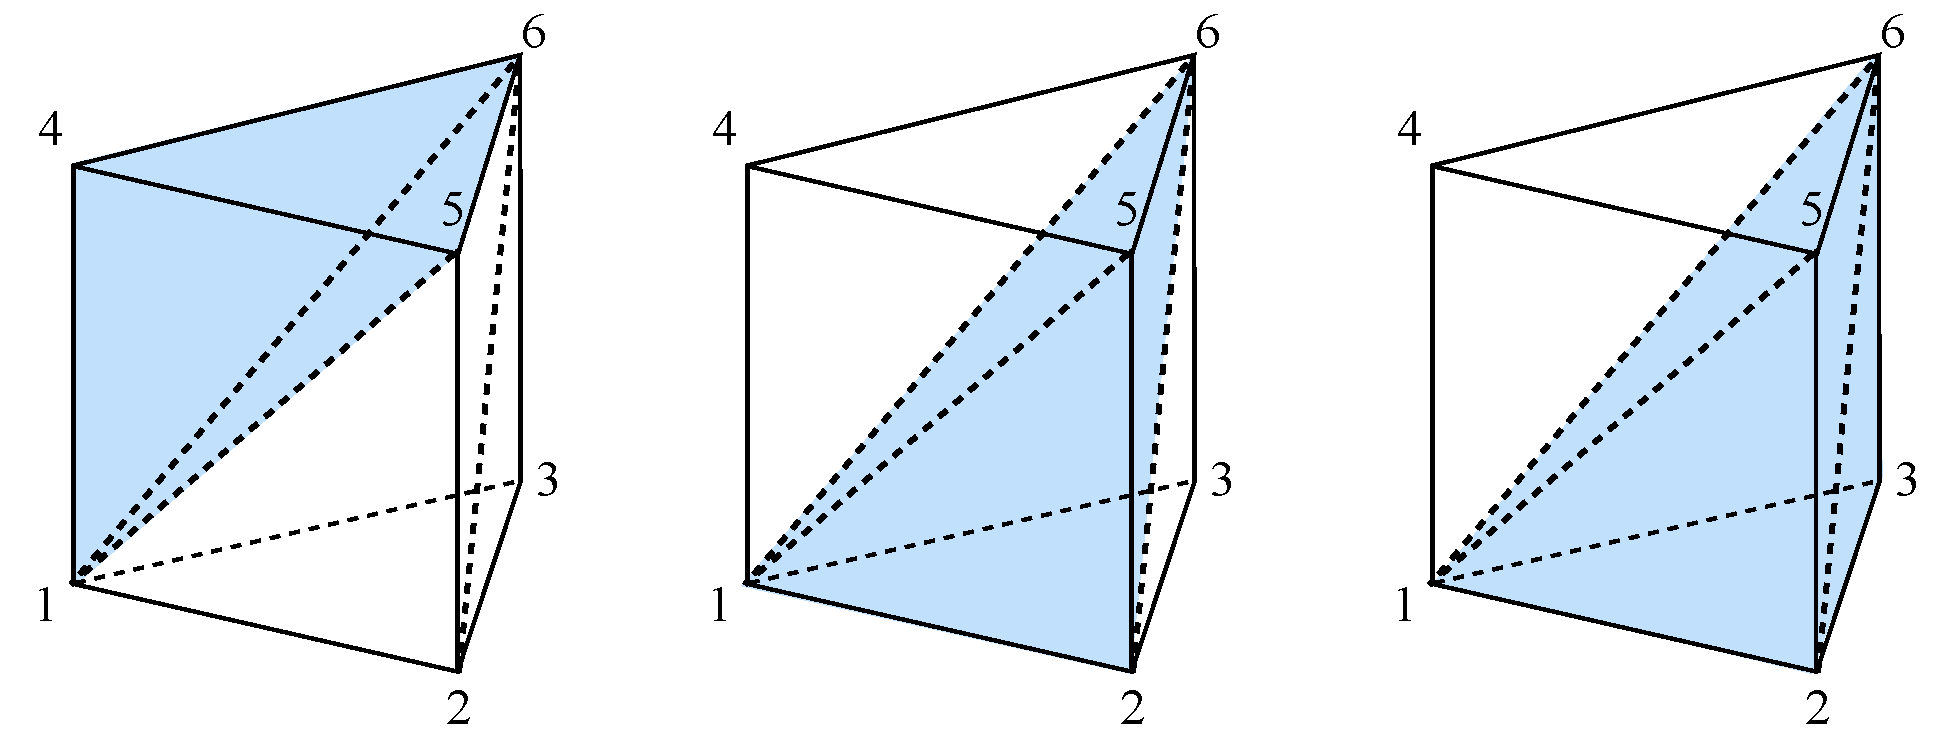
\includegraphics[scale=0.4]{graphics/prism_tetra.pdf}%
\caption{Decomposition of a prism into three tetrahedra.}%
\label{decoupage prisme}%
\end{figure}


\begin{CommentBlock}{Important remark:}
The diffusion matrix should only possess negative extra-diagonal terms
and the sum of each line should always yield zero in order
to achieve monotonicity and conservation.
However, from the computational point of view the extra-diagonal terms
can happen to be positive. Thus, the diffusion matrix in TELEMAC-3D
is modified: all extra-diagonal terms are clipped to a maximum value
of zero and the diagonal terms are modified so as to always retrieve
a zero-sum of each line. %Thus, monotonicity and conservation are ensured.
\end{CommentBlock}

With distributive schemes or when the user chooses to explicit the
diffusion ($\theta_d=0$), the first term in the left-hand side is mass-lumped
and \eqref{eq:diff} reads:
\begin{equation}
\begin{array}{ll}
\vec{u}_j^D\displaystyle{\int_\Omega}\vec{\Psi}_i~d\Omega +
\delta t \theta_d\nu_{Ej}\vec{u}_j^D\displaystyle{\int_\Omega}\Grad\vec{\Psi}_i
:\Grad\vec{\Psi}_j~d\Omega & = \vec{u}_j^A\displaystyle{\int_\Omega}
\vec{\Psi}_i\vec{\Psi}_j~d\Omega \bigskip \\
& ~\hspace{-4cm}+\delta t (1-\theta_d)\vec{u}_j^A\displaystyle{\int_\Omega}
\vec{\Psi}_i\Div(\nu_{Ej}\Grad\vec{\Psi}_j)~d\Omega
+\displaystyle{\int_\Gamma}\nu_{E}\Grad\vec{u}^D\cdot\vec{\Psi}_i\cdot\vec{n}
~d\Gamma
\end{array}
\end{equation}

\begin{CommentBlock}{Mass-lumping:}
The mass-lumping corresponds to a modification of a matrix
to obtain a diagonal matrix where all the extra-diagonal components
were summed onto the diagonal, line by line. This constitutes
an approximation of the original matrix but simplifies the
resolution of the system since only a division by the diagonal is
necessary.
\end{CommentBlock}

\begin{CommentBlock}{Remark:}
The calculation of $\displaystyle{\int_\Omega}\vec{\Psi}_i~d\Omega$ in the
left-hand side is done in agreement with the choice of mass-lumping for
the water heigth term in the wave equation (see the section
\ref{sec:masslumping}).
\end{CommentBlock}

\subsection{\label{calcul flottabilite 3D}Buoyancy terms%
\index{buoyancy}%
}

The source terms of buoyancy are one of the strategic points of 3D equations.
Their correct treatment conditions the representation of stratifications, a
current stumbling block of modelling. These source terms are, if we do not
consider atmospheric pressure (see the section \ref{sec:boussinesq}):%

\begin{equation}
F_{x}=g\dfrac{\Delta\rho}{\rho_{o}}\left(  \dfrac{\partial \eta}{\partial
x}\right)  _{y,t}-g\dfrac{\partial}{\partial x}\left(  \int\nolimits_{z}%
^{\eta}\dfrac{\Delta\rho}{\rho_{o}}\,dz\right)  _{y,z,t}%
\end{equation}
%
\begin{equation}
F_{y}=g\dfrac{\Delta\rho}{\rho_{o}}\left(  \dfrac{\partial \eta}{\partial
y}\right)  _{x,t}-g\dfrac{\partial}{\partial y}\left(  \int\nolimits_{z}%
^{\eta}\dfrac{\Delta\rho}{\rho_{o}}\,dz\right)  _{x,z,t}%
\end{equation}
%
The terms $F_{x}$ and $F_{y}$ are calculated on the mesh at time $t^{n}$ on
the basis of differences in density $\Delta\rho$. These differences in density
themselves have been evaluated earlier with the help of a state function in
which the different concentrations of active scalars appear.
Bijvelds \cite{bijvelds01} compares the treatment of these terms in sigma
transform formulation, in different software.
The term $F_{x}$ can be calculated either in the real mesh or in the transformed mesh.
In TELEMAC-3D, the calculation is done in the real mesh.
%Given below are two modes of
%calculation, limited to the term $F_{x}$, the first in the real mesh and the
%second in the transformed mesh.

\paragraph{Calculation in the real mesh:}

the second term of $F_{x}$\ cannot be directly expressed in the form of
vectors in finite elements. It has to be transformed with the Leibnitz formula
to obtain:%

\begin{equation}
-g\dfrac{\partial}{\partial x}\left(  \int\nolimits_{z}^{\eta}\dfrac{\Delta
\rho}{\rho_{o}}\,dz\right)  _{y,z,t}=-g\left[  \int\nolimits_{z}^{\eta}%
\dfrac{\partial}{\partial x}\left(  \dfrac{\Delta\rho}{\rho_{o}}\right)
\,dz+\dfrac{\Delta\rho(\eta)}{\rho_{o}}\dfrac{\partial \eta}{\partial x}\right]
\end{equation}


We finally get:%

\begin{equation}
F_{x}=-g\int\nolimits_{z}^{\eta}\dfrac{\partial}{\partial x}\left(
\dfrac{\Delta\rho}{\rho_{o}}\right)  \,dz+g\dfrac{\partial \eta}{\partial
x}\left(  \dfrac{\Delta\rho(z)}{\rho_{o}}-\dfrac{\Delta\rho(\eta)}{\rho_{o}%
}\right)
\end{equation}


This formula is simply calculated by using vertical lines of the mesh for the
integral along $z$ and to find the value of $\Delta\rho(\eta)$ above one point
of elevation $z$.

\begin{CommentBlock}{Remark:}
The Appendix B \ref{appendixB}
explains how these terms can be calculated in
the transformed mesh. TELEMAC-3D contains the corresponding code but it is not
used at the moment.
\end{CommentBlock}

\subsection{\label{friction3D}Friction terms%
\index{friction}%
}
Compatibility between friction terms in 2D and 3D is discussed in
\cite{hervouet007}; however, this is only valid for formulae relying on a
depth-integrated velocity, such as those of Strickler%
\index{Strickler!formula}
or Ch\'{e}zy%
\index{Ch\'{e}zy!formula}%
. If we want to use a local roughness factor and assume a logarithmic profile
near the bed, the friction velocity $u_{\ast}$ has to be evaluated. We can
use the fact that the mesh of prisms is made of piled-up meshes of triangles
and consider the first plane above the bed. If we assume that this first
plane is still in the logarithmic profile, we can write (the example of a
hydraulically rough flow):%
\index{rough flow}%
%
\begin{equation}
u_*=\dfrac{\kappa u_{plane\,1}}{\ln\left(\dfrac{33\Delta z}{k_{s}}\right)}%
\end{equation}
where $u_{plane\,1}$ is the velocity at the first point above the bed and
$\Delta z$ the altitude of this point above the bed.

\subsection{\label{calcul termes sources 3D}Other source terms}

The other source terms included in the terms $F_{x}$ and $F_{y}$\ are also
treated in the diffusion stage, explicitly (Coriolis, source points, culverts,
rain and evaporation, tidal forcing, etc.).

\section{\label{etape hydrostatique}Space discretisation of the hydrostatic step}
Here we only consider the case where the dynamic pressure is calculated after the resolution of
the hydrostatic step. We recall that we wrote the following system for the calculation of $h^{n+1}-h^{n}$ and
$\tilde{\vec{u}}_{2D}^{n+1}$ in the section \ref{Chapter3}:
\begin{equation}
  \left\{\begin{array}{l}
    \dfrac{h^{n+1}-h^{n}}{\delta t}
    + \nabla_{2D}\cdot \displaystyle{\int_b^\eta\left(\theta_u\tilde{\vec{u}}_{2D}^{n+1}+(1-\theta_u)\vec{u}_{2D}^n\right)~dz}=0 \medskip \\
    \dfrac{\tilde{\vec{u}}_{2D}^{n+1}-\vec{u}_{2D}^{A}}{\delta t}=-g \theta_h \Grad_{2D}(h^{n+1}-h^n) -g\Grad_{2D}\eta^n
     + \tilde{\vec{F}}_{2D}
     +\Div(\nu_E \Grad \vec{u}_{2D}) \medskip \\
  \end{array}\right.
\label{eq:systeme_hydrostatique}
\end{equation}
The time-discretisation for the diffusion term in the second line will be specified later.
In the sub-sections \ref{continuitytransformed} and \ref{momentumvariational},
a variational formulation for the depth-integrated
continuity equation (first line of this system) and for the horizontal momentum equation (second line)
are derived. The latter will provide an expression of $\tilde{\vec{u}}_{2D}^{n+1}$,
that is introduced in the first line in order to calculate $h^{n+1}$.
Once $h^{n+1}$ is known, the value of $\tilde{\vec{u}}_{2D}^{n+1}$ is retrieved through the horizontal
momentum equation. In between, a conservative velocity $\vec{u}_{2D}^C$ will have been calculated,
which is the one used for the advection terms.

%In the momentum equation, increments of the water depth are made to appear by
%a semi-implicitation of the free surface, like for the Saint-Venant equations:%
%
%\begin{equation}
%\begin{array}{l}
%\dfrac{\vec{u}^{C}-\vec{u}^{A}}{\delta t}= \\
%-s1u\,\,\vec{u}^{n+1}-g\theta_{h}\,\Grad%
%(h^{n+1}-h^{n})-g\,\Grad(\eta^{n})-\dfrac{1}{\rho
%}\Grad(p_{d})+\vec{F}+div(\nu_{t}%
%\Grad(\vec{u}))
%\end{array}
%\end{equation}
%\begin{WarningBlock}{Dynamic pressure + s1u source terms}
%The gradient of an estimated dynamic pressure can be included in the momentum equation at this stage.
%Describe it? It is an option right?
%Also, what to do with the s1u notation?
%\end{WarningBlock}


\subsection{\label{continuitytransformed}Variational formulation of the depth-integrated continuity equation in the transformed mesh}

The time-space discretised depth-averaged continuity equation is derived starting from the
continuity equation $\Div \vec{u}=0$ written in the transformed mesh
(see the equation \ref{divutransf}):
\begin{equation}
\dfrac{1}{\Delta z}\left[  \dfrac{\partial\Delta z}{\partial t}+\left(
\dfrac{\partial  \Delta z u  }{\partial x}\right)_{y,z^{\ast},t}
+\left(\dfrac{\partial \Delta z v }{\partial y}\right)_{x,z^{\ast},t}
+\left(\dfrac{\partial\Delta z w^{\ast}}{\partial z^{\ast}}\right)_{x,y,t}\right]
=0 \label{continuiteparplan}
\end{equation}
For each degree of freedom $i$ we should thus solve:
\begin{equation}
\displaystyle{\int_{\Omega^{\ast}}}\left[  \dfrac{\partial\Delta z}{\partial t}+\left(
\dfrac{\partial\Delta z u}{\partial x}\right)_{y,z^{\ast},t}+\left(
\dfrac{\partial\Delta z v}{\partial y}\right)_{x,z^{\ast},t}+\left(
\dfrac{\partial\Delta z w^{\ast}}{\partial z^{\ast}}\right)_{x,y,t}\right]
\Psi_{i}^{\ast}~d\Omega^{\ast}=0
\end{equation}
We shall go through the process of vertical integration of this equation, and then
of injection of the velocity coming from the momentum equation, to derive
the space-time discretised equation on $h^{n+1}-h^{n}$.
%With a simple sigma transform we would in fact get:
%\begin{equation}
%\displaystyle{\int_{\Omega^{\ast}}}\left[  \left(  \dfrac{\partial h}{\partial t}\right)
%_{x,y}+\left(  \dfrac{\partial hu}{\partial x}\right)  _{y,z^{\ast},t}+\left(
%\dfrac{\partial hv}{\partial y}\right)_{x,z^{\ast},t}+\left(  \dfrac{\partial
%hw^{\ast}}{\partial z^{\ast}}\right)_{x,y,t}\right]  \Psi_{i}^{\ast
%}d\Omega^{\ast}=0
%\end{equation}
%where we see the underlying depth-integrated continuity equation.
%It is actually this form of the mass conservation equation that is found while
%demonstrating the mass conservation of the scalar (see the section
%\ref{masse traceur}). Discretized as such, this equation whose unknown is
%$w^{\ast}$ or rather $\Delta z w^{\ast}$ leads to an ill-posed system.
%The boundary conditions are $w^{\ast}=0$ at the bottom and the free surface, if they are impermeable.
%The term:
%\begin{equation}
%\displaystyle{\int_{\Omega^{\ast}}}\left(
%\dfrac{\partial\Delta z w^{\ast}}{\partial z^{\ast}}\right)_{x,y,t}
%\Psi_{i}^{\ast}d\Omega^{\ast}
%\end{equation}
%with the unknown $\Delta z w^{\ast}$, leads to a matrix $A$ with general term:
%\begin{equation}
%A_{ij}=\displaystyle{\int_{\Omega^{\ast}}}\dfrac{\partial\Psi_{j}^{\ast}}{\partial z^{\ast}}
%\Psi_{i}^{\ast}d\Omega^{\ast}
%\end{equation}
%Recalling the structure of our basis, $\Psi_{i}^*=\Psi_{i}^{v*}(z)\Psi_{i}^H(x,y)$, the diagonal terms of this matrix thus read:
%\begin{equation}
%A_{ii}=\displaystyle{\int_{\Omega^{\ast}}}\dfrac{\partial}{\partial z^{\ast}}\left[\dfrac{{\Psi_{i}^{\ast}}^2}{2}\right]d\Omega^{\ast}=
%\left(\displaystyle{\int_{z^*=b}^{\eta}}\dfrac{\partial}{\partial z^{\ast}}\left[\dfrac{{\Psi_{i}^{v\ast}}^2}{2}\right]dz^{\ast}\right)
%\left(\displaystyle{\int_{\Omega_{2D}}}{\Psi_{i}^{h}}^2 d\Omega_{2D}\right) =
%\left[\Psi_{i}^{v\ast}\right]_{b}^{\eta}
%\end{equation}
%Outside the bed and free-surface boundaries, the diagonal terms of this matrix are thus equal to zero
%and the matrix is not invertible.
%%From the
%%boundary conditions at the bottom and the free surface, we arrive at
%%disconnected solutions between two successive planes (parasitic oscillations),
%%or an impossibility.
%This is because the only unknown retained for solving
%mass conservation is the vertical velocity. The figure \ref{probleme surcontraint}
%shows the case of a mesh reduced to two planes, where no degree of freedom is
%available on the vertical $i$ to find a vertical velocity for re-establishing
%a divergence-free flow.
%
%\begin{figure}[tbh]%
%\centering
%\includegraphics[
%natheight=2.330700in,
%natwidth=3.240400in,
%height=2.1257in,
%width=2.9456in
%]
%{NG0IDC07.wmf}
%\caption{example of a forced problem}
%\label{probleme surcontraint}
%\end{figure}
%
%A vertical velocity defined on a staggered mesh would be necessary, as show in
%the figure \ref{vitesse verticale}.
%\begin{figure}[tbh]
%\centering
%\includegraphics[natheight=2.330700in,
%natwidth=3.240400in,
%height=2.1257in,
%width=2.9456in]
%{NG0IDC08.wmf}
%\caption{the corresponding vertical velocity}
%\label{vitesse verticale}
%\end{figure}
%
%To circumvent this problem, a solution consists of changing the unknown or, to
%be more accurate, of giving a specific definition of the unknown $\Delta
%zw^{\ast}$. This definition, which will be given in the next paragraph, has
%been inspired by the necessity to get an exact mass conservation of scalars
%with distributive schemes. As a matter of fact, it will in due course appear
%that this definition of $\Delta zw^{\ast}$ is entirely compatible with these
%distributive schemes.
%
%Observing that, at the continuous level:
%\begin{equation}
%\begin{array}{ll}
%\theta_{u}\vec{u}^{C}+(1-\theta_{u})\vec{u}^{n}&=
%\theta_{u}D^{-1}\left(\vec{u}^{A}+\delta t\left[\vec{F}-\vec{diff}
%-g\Grad\eta^{n}-\dfrac{1}{\rho}\Grad p_{d}\right]\right)\\ \bigskip
%& +(1-\theta_{u})\vec{u}^{n}-\delta t D^{-1}g\theta_{h}\theta_{u}\Grad\delta h
%\end{array}
%\end{equation}
A variational formulation of the 3D continuity equation in the transformed mesh
(equation \ref{divutransf}) can be written in the form:
\begin{equation}
\begin{array}{ll}
\dfrac{1}{\delta t}\displaystyle{\int_{\Omega^{\ast}}}\left(\Delta z^{n+1}-\Delta z^{n}\right)\Psi_{i}^{\ast}~d\Omega^{\ast} & =
FLUINT(i)+FLUVER(i) \\ \medskip
& -FLUEXT(i)+SOURCE(i) \label{contidistr}
\end{array}
\end{equation}
with the following notations:
\begin{equation}
FLUINT(i)=\displaystyle{\int_{\Omega^{\ast}}}\Delta z\vec{u}
\cdot\Grad_{2D}\Psi_{i}^{\ast}~d\Omega^{\ast}
\end{equation}

\begin{equation}
FLUVER(i)=\int_{\Omega^{\ast}}\Delta zw^{\ast}\dfrac{\partial\Psi_{i}^{\ast}%
}{\partial z^{\ast}}~d\Omega^{\ast}%
\end{equation}

\begin{equation}
SOURCE(i)=\dfrac{\int\nolimits_{\Omega}Q_{sce}\Psi_{isce}\Psi_{i}\,d\Omega
}{\int\nolimits_{\Omega}\Psi_{isce}\,d\Omega}\alpha(i)
\end{equation}
%
\begin{equation}
FLUEXT(i)=\int\nolimits_{\Gamma_{liq}^{\ast}}\Delta z\vec{u}%
\cdot\vec{n}\Psi_{i}^{\ast}~d\Gamma^{\ast}%
\end{equation}

For all the degrees of freedom $i$. $\vec{u}\cdot\Grad_{2D}$ means that
only the first two components of the 3D velocity are taken into account.
The velocity $\vec{u}$ is here:%
\begin{equation}
\vec{u}=\theta_{u}\tilde{\vec{u}}^{n+1}+(1-\theta_{u})\vec{u}^{n}
\end{equation}
%\bigskip Our previous 2D continuity equation:
%\begin{equation}
%\dfrac{h^{n+1}-h^{n}}{\delta t}+div(h\left[  \theta_{u}\vec{u}%
%^{n+1}+(1-\theta_{u})\vec{u}^{n}\right]  )=Sce
%\end{equation}
%
%is now replaced by a sum on the vertical of the 3D continuity equations:%
Let us now sum these integrals over the degrees of freedom located above each $i$ of the 2D domain.
It is actually easier to write the first term in the real domain $\Omega$ to simplify it.
By definition of $\Delta z$, we have:
\begin{equation}
\displaystyle{\int_{\Omega}}\Psi_i~d\Omega=
\displaystyle{\int_{\Omega^*}}\Psi_i^*\dfrac{\partial z}{\partial z *}~d\Omega^*=
\displaystyle{\int_{\Omega^*}}\Psi_i^*\Delta z~d\Omega^*
\end{equation}
Let us sum all the values of $\displaystyle{\int_{\Omega}}\Psi_id\Omega$
along the degrees of freedom $j$ on the vertical of $i$:
\begin{equation}
\begin{array}{ll}
\displaystyle{\sum_{j~above~i}}\left(\displaystyle{\int_{\Omega}}\Psi_j~d\Omega\right)&=
\displaystyle{\sum_{j~above~i}}\left(\displaystyle{\int_{\Omega_{2D}}}\left(\displaystyle{\int_{z=b}^{\eta}}\Psi_j^V~dz\right)\Psi_i^H~d\Omega_{2D}\right)\bigskip\\
& = \displaystyle{\int_{\Omega_{2D}}}\left(\displaystyle{\int_{z=b}^{\eta}}\displaystyle{\sum_{j~above~i}}\Psi_j^V~dz\right)\Psi_i^H~d\Omega_{2D}\bigskip\\
& = \displaystyle{\int_{\Omega_{2D}}}h\Psi_i^H~d\Omega_{2D}
\end{array}
\end{equation}
The integral and sum symbols commute because the basis functions are always positive.
The first term of the equation \eqref{contidistr} thus becomes:
\begin{equation}
\begin{array}{ll}
\dfrac{1}{\delta t}\displaystyle{\int_{\Omega^{\ast}}}\left(\Delta z^{n+1}-\Delta z^{n}\right)\Psi_{i}^{\ast}~d\Omega^{\ast} &=
\dfrac{1}{\delta t}\displaystyle{\int_{\Omega_{2D}}}(h^{n+1}-h^n)\Psi_i^H~d\Omega_{2D}
%\dfrac{1}{\delta t}\displaystyle{\int_{z=0}^1}\left(\displaystyle{\int_{\Omega^*}}
%\left(\Delta z^{n+1}-\Delta z^{n}\right)\Psi_{i}^{*}d\Omega\right)&=
%\dfrac{1}{\delta t}\displaystyle{\sum_{j~above~i}}\left(\displaystyle{\int_{\Omega^*}}
%\left(\Delta z^{n+1}-\Delta z^{n}\right)\Psi_{j}^{*}d\Omega\right)\\\bigskip
%& = \dfrac{1}{\delta t}\displaystyle{\sum_{j~above~i}}\left(\displaystyle{\int_{\Omega^*}}
%\left(\Delta z^{n+1}-\Delta z^{n}\right)\Psi_{j}^{*V}\Psi_i^Hd\Omega\right)\\\bigskip
%& = \dfrac{1}{\delta t}\displaystyle{\sum_{j~above~i}}\left(\displaystyle{\int_{\Omega_{2D}}}\left(
%\displaystyle{\int_{z=0}^1}\left(\Delta z^{n+1}-\Delta z^{n}\right)\Psi_{j}^{*V}\right)\Psi_i^Hd\Omega_{2D}\right)\\\bigskip
%& \textcolor{red}{= \dfrac{1}{\delta t}\displaystyle{\int_{\Omega^*}}
%\displaystyle{\sum_{j~above~i}}\left(\Delta z^{n+1}-\Delta z^{n}\right)\Psi_{j}^{*V}\Psi_i^Hd\Omega}\\\bigskip
%& \textcolor{red}{= \dfrac{1}{\delta t}\displaystyle{\int_{\Omega_{2D}}}\left(\displaystyle{\int_{z=0}^1}
%\displaystyle{\sum_{j~above~i}}\left(\Delta z^{n+1}-\Delta z^{n}\right)\Psi_{j}^{*V}dz\right)\Psi_i^Hd\Omega_{2D}}\\\bigskip
%& = \dfrac{1}{\delta t}\displaystyle{\int_{\Omega_{2D}}}\left(h^{n+1}-h^n\right)\Psi_i^Hd\Omega_{2D}
\end{array}
\end{equation}
On the other hand, the term $FLUVER(i)$ sums to zero on a
vertical because of the properties of the basis function:
\begin{equation}
\begin{array}{ll}
\displaystyle{\sum_{j~above~i}}\displaystyle{\int_{\Omega^{\ast}}}\Delta zw^{\ast}
\dfrac{\partial\Psi_{j}^{\ast}}{\partial z^{\ast}}~d\Omega^{\ast} & =
\displaystyle{\sum_{j~above~i}}\displaystyle{\int_{\Omega^{\ast}}}\Delta zw^{\ast}
\dfrac{\partial\Psi_{j}^{v\ast}}{\partial z^{\ast}}\Psi_{i}^{h}~d\Omega^{\ast}%\\ \bigskip
%& = \displaystyle{\sum_{j~above~i}}\displaystyle{\int_{\Omega_{2D}}}\left(\displaystyle{\int_{z^*=0}^1}\Delta zw^{\ast}
%\dfrac{\partial\Psi_{j}^{v\ast}}{\partial z^{\ast}}dz^*\right)\Psi_{i}^{h}d\Omega_{2D}\\ \bigskip
%& = \displaystyle{\int_{\Omega^{\ast}}}\Delta zw^{\ast}
%\displaystyle{\sum_{j~above~i}}\dfrac{\partial\Psi_{j}^{v\ast}}{\partial z^{\ast}}\Psi_{j}^{h}d\Omega^{\ast}\\ \bigskip
%& = \displaystyle{\int_{\Omega^{\ast}}}\Delta zw^{\ast}\Psi_{j}^{h}
%\dfrac{\partial\left(\displaystyle{\sum_{j~above~i}}\Psi_{j}^{v\ast}\right)}{\partial z^{\ast}}d\Omega^{\ast}\\ \bigskip
%& = \displaystyle{\int_{\Omega^{\ast}}}\Delta zw^{\ast}\Psi_{j}^{h}
%\dfrac{\partial(1)}{\partial z^{\ast}}d\Omega^{\ast}\\ \bigskip
= 0
\end{array}
\end{equation}
\begin{figure}[t]
\begin{center}
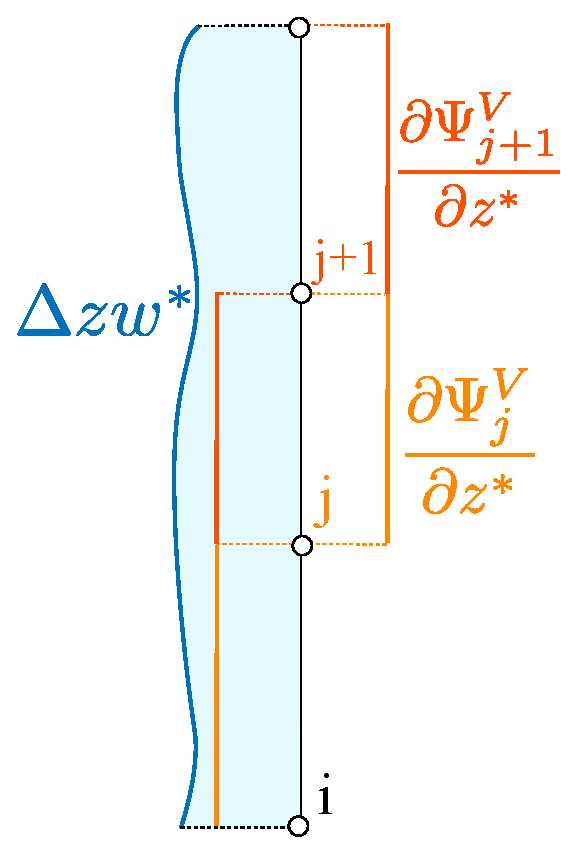
\includegraphics[scale=0.5]{graphics/fluvert.pdf}
\end{center}
\caption{Sketch of the cancellation of $\displaystyle{\sum_{j~above~i}}\displaystyle{\int_{\Omega^{\ast}}}\Delta zw^{\ast}
(\partial\Psi_{j}^{v\ast}/\partial z^{\ast})\Psi_{i}^{h}~d\Omega^{\ast}$: the
integral above a point $j$ cancels out with the one below $j+1$. The sum on
the whole vertical is thus equal to zero.}
\label{fig:fluvert}
\end{figure}
Indeed, the integrals cancel each other when summed along the vertical,
as shown in the figure \ref{fig:fluvert}.
The integration on the vertical of the equation \eqref{contidistr} thus reads:
\begin{equation}
\displaystyle{\int_{\Omega_{2D}}}\Psi_{i}^{h}\left(\dfrac{h^{n+1}-h^{n}}{\delta
t}\right)~d\Omega_{2D}+{\displaystyle\sum_{j~above~i}}
\left(-FLUINT(j)+FLUEXT(j)-SOURCE(j)\right)  =0
\end{equation}
or, more explicitely:%
\begin{equation}
\left[\begin{array}{l}
\displaystyle{\int_{\Omega_{2D}}}\Psi_{i}^{h}\left(\dfrac{h^{n+1}-h^{n}}{\delta
t}\right)~d\Omega_{2D}+
{\displaystyle\sum_{j~above~i}}FLUEXT(j)\\\bigskip
-\displaystyle{\sum_{j~above~i}}\int\nolimits_{\Omega^{\ast}}\Delta
z~\left(\theta_{u}\tilde{\vec{u}}^{n+1}+(1-\theta_{u})\vec{u}^{n}\right)\cdot\Grad^{\ast}\Psi_{j}^*~d\Omega^{\ast}
\end{array}\right]
={\displaystyle\sum_{j~above~i}}SOURCE(j)\label{eq:hequation}
\end{equation}

This corresponds to a variational formulation of the first
line of the equation \eqref{eq:hydrostatic_second_system}.

\begin{CommentBlock}{Remark:}
It is important to write a variational formulation and only then sum the integrals over the vertical,
otherwise the discrete conservation of mass is not achieved.
\end{CommentBlock}

\subsection{Estimation of the 2D conservative velocity}\label{momentumvariational}
In what follows, we want to obtain a formula to calculate $\tilde{\vec{u}}^{n+1}$ that
not involve having to solve a linear system: we need to then introduce
that formula into the equation \eqref{eq:hequation} to calculate $h^{n+1}$.
For this, we discretize the second line of the system \eqref{eq:wave_equation_time}, recalled below:
\begin{equation}
%  \dfrac{\tilde{\vec{u}}_{2D}^{n+1}-\vec{u}_{2D}^{A}}{\delta t}=-g \theta_h \Grad_{2D}(h^{n+1}-h^n) -g\Grad_{2D}\eta^n
%  + \tilde{\vec{F}}_{2D}
%  +\Div(\nu_E \Grad \vec{u}_{2D})
\dfrac{\vec{u}_{2D}^{aux}-\vec{u}_{2D}^{A}}{\delta t}= -g\Grad_{2D}\eta^n
     + \tilde{\vec{F}}_{2D}
     +\nu_E \Lap \vec{u}_{2D}\medskip\\
\end{equation}
Here the time discretisation of the diffusion term has not been specified: it is going to be specified below.
Recall that we then have:
\begin{equation}
 \tilde{\vec{u}}_{2D}^{n+1}=\vec{u}_{2D}^{aux}-g \theta_h \delta t\Grad_{2D}(h^{n+1}-h^n)
\end{equation}
We leave the framework of Finite Elements in this section, since we do not
write a variational formulation of the equation but rather use or compute nodal
values of each term so as to obtain $\vec{u}_{2D}^{aux}$ and then $\tilde{\vec{u}}_{2D}^{n+1}$.
The gradient term $-g\theta_{h}\Grad_{2D}(h^{n+1}-h^{n})$,
written also $-g\theta_{h}\Grad_{2D}\delta h$, shall be kept
in this continuous form when being introduced in the depth-integrated continuity equation.
When necessary, the nodal values of the fields or their gradients are estimated
with the following formula:
\begin{equation}
\left[f\right]_i\approx\dfrac{\displaystyle{\int_\Omega} f\Psi_i~d\Omega}{\displaystyle{\int_\Omega}\Psi_i~d\Omega}\label{eq:nodalvalue}
\end{equation}
or for a 2D field:
\begin{equation}
\left[f\right]_i\approx\dfrac{\displaystyle{\int_{\Omega_{2D}}}f\Psi_i~d\Omega_{2D}}{\displaystyle{\int_{\Omega_{2D}}}\Psi_i~d\Omega_{2D}}\label{eq:nodalvalue2D}
\end{equation}
Note that this is only an approximation of the nodal value of $f$.
Using this technique for the diffusion term yields:
\begin{equation}
\dfrac{\displaystyle{\int_{\Omega}}\Div(\nu_{E}\Grad\vec{u})\Psi_{i}~d\Omega}
{\displaystyle{\int_{\Omega}}\Psi_{i}~d\Omega}
\end{equation}
a form in which the discretisation in time is still not specified since we
wish to retain the friction terms in an implicit form and the volumic term in an
explicit, semi-implicit or implicit form.
An integration by parts of the numerator yields:
\begin{equation}
\displaystyle{\int_{\Omega}}\Div(\nu_{E}\Grad\vec{u}_{2D})\Psi_{i}~d\Omega=
\displaystyle{\int_{\Gamma}}\Psi_{i}\nu_{E}\Grad\vec{u}_{2D}\cdot\vec{n}~d\Gamma-
\displaystyle{\int_{\Omega}}\nu_{E}\Grad\vec{u}_{2D}\cdot\Grad\Psi_{i}~d\Omega
\end{equation}
Let us consider that the volumic
term is treated explicitly for the sake of simplicity.
The boundary term is treated implicitely.
The above equation then becomes:
\begin{equation}
\displaystyle{\int_{\Omega}}\Div(\nu_{E}\Grad\vec{u}_{2D})\Psi_{i}~d\Omega\simeq
\displaystyle{\int_{\Gamma}}\Psi_{i}\nu_{E}\Grad\vec{u}_{2D}^{aux}\cdot\vec{n}~d\Gamma
-\displaystyle{\int_{\Omega}}\nu_{E}\Grad\vec{u}_{2D}^{n}\cdot\Grad\Psi_{i}~d\Omega
\end{equation}
Now to deal with $\nu_{E}\Grad\vec{u}_{2D}^{aux}\cdot\vec{n}$ we write that:
\begin{equation}
\nu_{E}\Grad u^{aux}\cdot\vec{n}=aubor~u^{aux}+bubor
\end{equation}
and:
\begin{equation}
\nu_{E}\Grad v^{aux}\cdot\vec{n} = avbor~v^{aux}+bvbor
\end{equation}
$avbor=aubor$ represents the stress due to friction and $bubor$ and $bvbor$ an
explicit stress due for example to wind at the free surface or any other
stress at the bed or the lateral boundaries.
The term $\int_{\Gamma}\Psi_{i}\nu_{E}\Grad\vec{u}_{2D}^{aux}\cdot\vec{n}~d\Gamma$
finally takes the form of a diagonal matrix multiplied
by the velocity vector plus an explicit stress denoted by $\vec{bubor}$,
with components $bubor$ and $bvbor$. We now
estimate the nodal value of $aubor~\vec{u}_{2D}^{aux}$ with the formula
\eqref{eq:nodalvalue} and define $fric3d$ as:
\begin{equation}
\dfrac{\displaystyle{\int_{\Gamma}}\Psi_{i}~aubor~\vec{u}_{2D}^{aux}~d\Gamma}
{\displaystyle{\int_{\Omega}}\Psi_{i}~d\Omega}=-fric3d~\vec{u}_{2D}^{aux}
\end{equation}
We then use mass-lumping on $fric3d$ so as to have:
\begin{equation}
fric3d\simeq-\dfrac{\displaystyle{\int_{\Gamma}}\Psi_{i}~d\Gamma}
{\displaystyle{\int_{\Omega}}\Psi_{i}~d\Omega} aubor =
-\dfrac{aubor}{cos(\alpha)}~\dfrac{\displaystyle{\int_{\Omega_{2D}}}\Psi_{i}^{h}~d\Omega_{2D}}
{\displaystyle{\int_{\Omega}}\Psi_{i}~d\Omega}%
\end{equation}

Indeed, $1/cos(\alpha)$ is equal to $\sqrt{1+\left(\partial b/\partial x\right)^{2}+\left(\partial b/\partial y\right)^{2}}$
and as a matter of fact, we have:
\begin{equation}
d\Gamma=\sqrt{1+\left(\dfrac{\partial b}{\partial x}\right)^{2}
+\left(\dfrac{\partial b}{\partial y}\right)^{2}}d\Omega_{2D}
\end{equation}
on the bed, because the 2-dimensional domain is flat, whereas there is a
slope of the 2-dimensional boundary of the 3-dimensional domain.
On the other hand, we estimate the nodal value of $\nu_{E}\Grad\vec{u}_{2D}^{n}$
with the formula \eqref{eq:nodalvalue} and define $\vec{diff}$ as:
\begin{equation}
\vec{diff}=\dfrac{\displaystyle{\int_{\Omega}}\nu_{E}\Grad\vec{u}_{2D}^{n}
\cdot\Grad\Psi_{i}~d\Omega}{\displaystyle{\int_{\Omega}}\Psi_{i}~d\Omega}
-\vec{bubor}\dfrac{\displaystyle{\int_{\Gamma}}\Psi_{i}~d\Gamma}
{\displaystyle{\int_{\Omega}}\Psi_{i}~d\Omega}
\end{equation}
The nodal values of $\vec{bubor}$ were also approximated and a mass-lumping
was used to extract it from the integral, like for $\vec{aubor}$.
Finally, we estimate the diffusion term as:
\begin{equation}
\dfrac{\displaystyle{\int_{\Omega}}\Div(\nu_{E}\Grad\vec{u}_{2D})\Psi_{i}~d\Omega}
{\displaystyle{\int_{\Omega}}\Psi_{i}~d\Omega}\approx
-fric3d~\vec{u}_{2D}^{aux}-\vec{diff}
\end{equation}
%The expression of $\vec{u}^{C}$ carried over in the mass
%conservation equation will be:
%\begin{equation}
%\vec{u}^{C}=D^{-1}\left(\vec{u}^{A}+\delta t\left[-g\theta_{h}\Grad\delta h-g\Grad\eta^{n}
%-\dfrac{1}{\rho}\Grad p_{d}+\vec{F}-\vec{diff}\right]\right)
%\label{finalvel}
%\end{equation}

The expression of $\tilde{\vec{u}}_{2D}^{n+1}$ to be injected in the equation
\eqref{eq:hequation} then reads:
\begin{equation}
\tilde{\vec{u}}_{2D}^{n+1}=D^{-1}\left(\vec{u}_{2D}^{A}+\delta t\left[-g\theta_{h}\Grad_{2D}
\delta h^{n+1}+\dfrac{\displaystyle{\int_{\Omega_{2D}}}[-g\Grad_{2D}\eta^{n}]
\Psi_{i}^{h}~d\Omega_{2D}}{\displaystyle{\int_{\Omega_{2D}}}\Psi_{i}^{h}~d\Omega_{2D}}
+\vec{P}_{2D}+\vec{F}_{2D}-\vec{diff}\right]\right)\label{eq:uc}
\end{equation}
%while after the calculation of $\delta h$, $\vec{u}_{2D}^{C}$ is calculated
%through the formula:
%\begin{equation}
%\vec{u}_{2D}^{C}=D^{-1}\left(\vec{u}_{2D}^{A}+\delta t\left[
%\dfrac{\displaystyle{\int_{\Omega_{2D}}}[-g\theta_{h}\Grad_{2D}\delta h-g\Grad_{2D}
%\eta^{n}]\Psi_{i}^{h}d\Omega_{2D}}{\displaystyle{\int_{\Omega_{2D}}}\Psi_{i}^{h}
%d\Omega_{2D}}+\vec{P}_{2D}+\vec{F}_{2D}-\vec{diff}\right]\right)\label{eq:uc}
%\end{equation}
with:
\begin{equation}
D=1+\delta t(fric3d+s1u)
\end{equation}
with the explicit treatment of the volumic integral for the diffusion term, we have:
\begin{equation}
D^{-1}=\dfrac{1}{1+\delta t(fric3d+s1u)}%
\end{equation}
but it is intentionally kept in the form $D^{-1}$ because $D$ will become a
matrix when an implicit diffusion is taken into account (see the Finite Elements
discretisation of the diffusion step described in the equation \eqref{eq:diff}
for a better understanding of the implicit treatment of the diffusion).
$\vec{P}_{2D}$ stands for $-\int_{\Omega}1/\rho\Grad_{2D} p_{d}\Psi_{i}~d\Omega$.
%\textcolor{red}{Not divided by a psi integral??}
%We thus have an equation for the calculation of $\vec{u}^{C}$.

In the equation \eqref{eq:uc}, $\Grad_{2D}\delta h^{n+1}$ is calculated as
a nodal value, like $-g\,\Grad_{2D}\eta^{n}$, that is:%
\begin{equation}
\dfrac{\displaystyle{\int_{\Omega_{2D}}}[-g\theta_{h}\Grad_{2D}\delta
h^{n+1}-g\Grad_{2D}\eta^{n}]\Psi_{i}^{h}~d\Omega_{2D}}
{\displaystyle{\int_{\Omega_{2D}}}\Psi_{i}^{h}~d\Omega_{2D}}
\end{equation}
This is provisional, we will see in the next subsection that in the continuity
equation $\Grad_{2D}\eta^{n}$ can be treated differently suppress wiggles.

%Assuming that an advection step (explicit or method of characteristics) has
%earlier given a velocity field $\vec{u}^{C}$ the momentum equation is:%
%
%\begin{equation}
%\dfrac{\vec{u}^{n+1}-\vec{u}^{C}}{\delta t}%
%=-s1u\,\,\vec{u}^{n+1}-g\,\Grad(\eta)-\dfrac
%{1}{\rho}\Grad(p_{d})+\vec{F}+div(\nu
%_{t}grad(\vec{u}))
%\end{equation}
%
%where $\vec{F}$ specifically contains the buoyancy terms, that is:%
%
%\begin{equation}
%\vec{F}=g\dfrac{\Delta\rho}{\rho_{o}}\Grad%
%(\eta)-g\,\Grad\left(  \int\nolimits_{z}^{\eta}\dfrac
%{\Delta\rho}{\rho_{o}}dz^{\prime}\right)
%\end{equation}
%
%The term $-s1u\,\,\vec{u}^{n+1}$represents the manner in which any
%possible implicit source terms are treated. $s1u$ is a function discretised as
%the velocity.


\subsection{Variational formulation of the equation on $h^{n+1}$ - pseudo wave equation}

We have defined:
\begin{equation}
\vec{u}^{aux}=D^{-1}\left(\vec{u}_{2D}^{A}+\delta t\left[-
\dfrac{\displaystyle{\int_{\Omega_{2D}}}g\Grad_{2D}\eta^{n}\Psi_{i}^{h}~d\Omega_{2D}}
{\displaystyle{\int_{\Omega_{2D}}}\Psi_{i}^{h}~d\Omega_{2D}}
+\vec{P}_{2D}+\vec{F}_{2D}-\vec{diff}\right]\right)\label{UAUX}
\end{equation}
The depth-integrated continuity equation in variational formulation is then written as:
\begin{equation}
\begin{array}{l}
\displaystyle{\int_{\Omega_{2D}}}\Psi_{i}^{h}\left(\dfrac{h^{n+1}-h^{n}}{\delta t}\right)~d\Omega_{2D}
+g\delta t\theta_{h}\theta_{u}\displaystyle{\sum_{j~above~i}}
\left(\displaystyle{\int_{\Omega^{\ast}}}\Delta z~D^{-1}\Grad(h^{n+1}-h^{n})\cdot\Grad\Psi_{j}^{*}~d\Omega^{\ast}\right)=\\\medskip
\displaystyle{\sum_{j~above~i}}
\left(\displaystyle{\int_{\Omega^{\ast}}}\Delta z~
\left(\theta_{u}\vec{u}^{aux}+(1-\theta_{u})\vec{u}^{n}\right)
\cdot\Grad\Psi_{j}^{*}~d\Omega^{\ast}\right)+\displaystyle{\sum_{j~above~i}}\left[  SOURCE(j)-FLUEXT(j)\right]
\end{array}
\end{equation}
where the variational formulation for the term containing $\delta h$ in the conservative velocity is
now consistent with the rest of the water-depth equation -- a 3D integration followed by a summation on
the vertical of each degree of freedom.
The second term in the left-hand side is written as:
\begin{equation}
\begin{array}{l}
g\delta t\theta_{h}\theta_{u}\displaystyle{\sum_{j~above~i}}
\left(\displaystyle{\int_{\Omega^{\ast}}}\Delta z~D^{-1}\Grad(h^{n+1}-h^{n})\cdot\Grad\Psi_{j}^{*}~d\Omega^{\ast}\right)=%\\\bigskip
%g\delta t\theta_{h}\theta_{u}
%\displaystyle{\int_{\Omega_{2D}}}\left(\displaystyle{\sum_{j~above~i}}\Delta z~D^{-1}\right)\Grad(h^{n+1}-h^{n})\cdot\Grad\Psi_{i}^{h}d\Omega^{\ast}=%\\\bigskip
\displaystyle{\int_{\Omega_{2D}}}\nu_{wave}\Grad(h^{n+1}-h^{n})\cdot\Grad\Psi_{i}^{h}~d\Omega^{\ast}
\end{array}
\end{equation}
%\bigskip The term:%
%\begin{equation}
%\int_{\Omega^*}\left[\delta tD^{-1}g\theta_{h}\theta_{u}\Grad(h^{n+1}-h^{n})\right] \cdot
%\Grad\Psi_{i}^{h}d\Omega^*
%\end{equation}
%is written:%
%\begin{equation}
%\int\nolimits_{\Omega_{2D}}\nu_{wave}~\Grad(h^{n+1}%
%-h^{n})\,.\Grad(\Psi_{i}^{h})\,d(\Omega_{3D})
%\end{equation}
where $\nu_{wave}$ is a piece-wise constant function equal to:%
\begin{equation}
\nu_{wave}(ielem)=g\delta t~\theta_{h}\theta_{u}\sum_{prisms~above~ielem}
\overline{(\Delta zD^{-1})} \label{nuwave}%
\end{equation}
where the bar stands for an average on the prism. $ielem$ is a 2D element
number.

\begin{CommentBlock}{Remark:}
The choice of $\nu_{wave}$ as a piece-wise constant function stems
from the fact that when summed over the vertical, the terms:%
\begin{equation}
\sum_{j~above~i}\int_{\Omega^{\ast}}\Delta zg\delta t
\theta_{h}\theta_{u}D^{-1}\Grad(h^{n+1}-h^{n})\cdot\Grad\Psi_{j}^*~d\Omega^{\ast}
\end{equation}
should give:
\begin{equation}
\int_{\Omega_{2D}}\nu_{wave}\Grad(h^{n+1}-h^{n})\cdot\Grad\Psi_{i}^{h}~d\Omega_{2D}
\end{equation}
In this way the treatment of this term is simpler and we
recover a Saint-Venant like continuity equation.
If we consider the integral:
\begin{equation}
\int_{\Omega^{\ast}}\Delta z~g\delta t\theta_{h}\theta_{u}D^{-1}\Grad(h^{n+1}-h^{n})
\cdot\Grad\Psi_{j}^{*}~d\Omega^{\ast}
\end{equation}
on a prism, the only real 3-dimensional function is $\Delta z~D^{-1}$, so that
$\Delta z~D^{-1}$ can be replaced by its average on the prism $\overline
{\Delta z~D^{-1}}$ without changing the result. Then by summing over the
vertical we get to:
\begin{equation}
\int_{\Omega_{2D}}\nu_{wave}\Grad(h^{n+1}-h^{n})\cdot\Grad\Psi_{i}^{h}~d\Omega_{2D}
\end{equation}
%if we take $\nu_{wave}$ defined by the equation \ref{nuwave}.
\end{CommentBlock}


Finally, the variational formulation of the equation on $h^{n+1}$ reads:%
\begin{equation}
\begin{array}{l}
\displaystyle{\int_{\Omega_{2D}}}\left(\dfrac{h^{n+1}-h^{n}}{\delta t}\right)\Psi_{i}^{h}~d\Omega_{2D}
+\displaystyle{\int_{\Omega_{2D}}}\nu_{wave}\Grad(h^{n+1}-h^{n})\cdot\Grad\Psi_{i}^{h}~d\Omega_{2D}=\bigskip\\
\displaystyle{\sum_{j~above~i}}\left(\displaystyle{\int_{\Omega^{\ast}}}
\Delta z (\theta_{u}\vec{u}^{aux}+(1-\theta_{u})\vec{u}^{n})\cdot\Grad\Psi_{j}^{*}~d\Omega^{\ast})\right)
+\displaystyle{\sum_{j~above~i}}\left(  SOURCE(j)-FLUEXT(j)\right)
\end{array}
\label{contiwave}%
\end{equation}
and $\vec{u}_{2D}^{C}$ is calculated through:
\begin{equation}
\vec{u}_{2D}^{C}=\theta_u\vec{u}_{2D}^{aux}+(1-\theta_u)\vec{u}_{2D}^n
\label{eq:ucfinal}
\end{equation}
%and the variational formulation of the momentum equation is:%
%\begin{equation}
%\vec{u}_{2D}^{C}=\vec{u}^{aux}-\delta tD^{-1}\left[
%\dfrac{\int_{\Omega_{2D}}g\theta_{h}\Grad_{2D}(h^{n+1}-h^{n})\Psi_{i}^{h}d\Omega_{2D}}
%{\int_{\Omega_{2D}}\Psi_{i}^{h}d\Omega_{2D}}\right] \label{finalvelocity}%
%\end{equation}

%\clearpage
%%%%%%%%%%%%%%%%%%%%%%%%%%%%%%%%%%%%%%%%%%%%%%%%%%%%%%%%%%%%%%%
\begin{CommentBlock}{Remark:}
In case the gradient of the dynamic pressure is included in $\vec{u}^{aux}$,
a term $-(1/\rho)\Grad p_{d}$ is added to
the momentum equation, where $p_{d}$ is calculated by applying the Chorin
projection method before calculating the new water depth.
This corresponds to the key-word \texttt{DYNAMIC PRESSURE IN WAVE EQUATION}
(see the section \ref{sec:dynamicpressureinwaveequation}).
\end{CommentBlock}
%%%%%%%%%%%%%%%%%%%%%%%%%%%%%%%%%%%%%%%%%%%%%%%%%%%%%%%%%%%%%%%
\\

%%%%%%%%%%%%%%%%%%%%%%%%%%%%%%%%%%%%%%%%%%%%%%%%%%%%%%%%%%%%%%%
\begin{CommentBlock}{Some history:}
In former versions of TELEMAC-3D this step was solved by
calling TELEMAC-2D. It then appeared that this was a theoretical
mistake: average on the vertical and discretisation do not commute. The right
thing to do is to first discretise the equations in 3D, then to sum them over
the vertical. This sum is thus discrete and done plane by plane. In the more
recent versions the only technique proposed is the wave equation, which
consists of eliminating the velocity from the depth-summed continuity equation,
yielding an equation on the depth, which looks like a wave equation as the celerity
of waves clearly appears in it.
\end{CommentBlock}

\subsubsection{Equivalence between the pseudo-wave equation and a Saint-Venant like continuity equation}
The continuity equation, given bed and free-surface boundary conditions,
yields a Saint-Venant like continuity equation. The classical version of the
Saint-Venant continuity equation is recalled below, with a variational formulation and a time discretisation:
\begin{equation}
\displaystyle{\int_{\Omega_{2D}}}\left(\dfrac{h^{n+1}-h^{n}}{\delta t}
\right)\Psi_{i}^{h}~d\Omega_{2D}
+\displaystyle{\int_{\Gamma_{2D}}}h\vec{U}\cdot\vec{n}\Psi_{i}^{h}~d\Gamma_{2D}
-\displaystyle{\int_{\Omega_{2D}}}h\vec{U}\cdot\Grad\Psi_{i}^{h}~d\Omega_{2D}=0
\end{equation}
The continuity equation solved to obtain the values of water height,
\eqref{contiwave}, can also be considered as:%
\begin{equation}
\begin{array}{l}
\displaystyle{\int_{\Omega_{2D}}}\left(\dfrac{h^{n+1}-h^{n}}{\delta t}
\right)\Psi_{i}^{h}~d\Omega_{2D}-\displaystyle{\sum_{j~above~i}}\left(
\displaystyle{\int_{\Omega^{\ast}}}\Delta z\vec{u}^{comp}\cdot\Grad\Psi_{j}^{*}
~d\Omega^{\ast}\right)\bigskip\\
-\displaystyle{\sum_{j~above~i}}\left(  SOURCE(j)-FLUEXT(j)\right)  =0
\end{array}
\end{equation}
with $\vec{u}^{comp}$ being here:
\begin{equation}
\vec{u}^{comp}=\theta_u\vec{u}^{aux}+(1-\theta_u)\vec{u}^n-g\delta t\theta_{h}\theta_{u}D^{-1}\Grad(h^{n+1}-h^{n})%=\theta_u\vec{u}^{C*}+(1-\theta_u)\vec{u}^n
\end{equation}
We have:
\begin{equation}
\displaystyle{\sum_{j~above~i}}\left(
\displaystyle{\int_{\Omega^{\ast}}}\Delta z\vec{u}^{comp}\cdot\Grad\Psi_{j}^{*}
~d\Omega^{\ast}\right)=\int_{\Omega_{2D}}\displaystyle{\sum_{j~above~i}}\Delta z\vec{u}^{comp}\cdot\Grad\Psi_j^H~d\Omega_{2D}
\end{equation}
For the same reason as $FLUEXT = 0$, so that the equation \eqref{contiwave}
is a form of depth-integrated continuity equation, as expected.

\subsubsection{Mass-lumping of the pseudo-wave equation}\label{sec:masslumping}

Mass-lumping may be used to solve the pseudo-wave equation.
It is always the case when distributive schemes are used for the advection,
otherwise it is a choice left to the user.
In case mass-lumping is used, the left-hand side of the equation
\eqref{contiwave} is approximated in the form:
\begin{equation}
\dfrac{1}{\delta t}\int\nolimits_{\Omega_{2D}}(h^{n+1}-h^{n})\Psi_{i}^{h}
~d\Omega_{2D}\simeq\dfrac{(h_{i}^{n+1}-h_{i}^{n})}{\delta t}\int%
\nolimits_{\Omega_{2D}}\Psi_{i}^{h}~d\Omega_{2D}%
\end{equation}
then the terms $\int\nolimits_{\Omega^{n+1}}\Psi_{i}~d\Omega^{n+1}$ and
$\int\nolimits_{\Omega^{n}}\Psi_{i}~d\Omega^{n}$ must be modified accordingly
everywhere they are used in the equations. Indeed, for a case like the one
shown in the figure \ref{fig:masslumping}, the integral of the basis
around $i$ is not equal to zero while $h_i$ is equal to 0, so that the
mass-lumped terms involving $h_i$ will cancel out but not the ones
involving other quantities. This leads to spurious mass transfers and must be avoided. As a matter of fact, we must write:%
\begin{equation}
\int\nolimits_{\Omega}\Psi_{i}~d\Omega=\int_{\Omega^{\ast}}h\Psi_{i}^{\ast
}~d\Omega^{\ast}\simeq h_{i}\int_{\Omega^{\ast}}\Psi_{i}^{\ast}~d\Omega^{\ast}%
\label{eq:volu}
\end{equation}
In this way, the calculation the diffusion stage (for the vertical velocity and
scalars) and the velocity correction stage remain compatible
with the mass-lumped pseudo wave equation.

\begin{figure}
\begin{center}
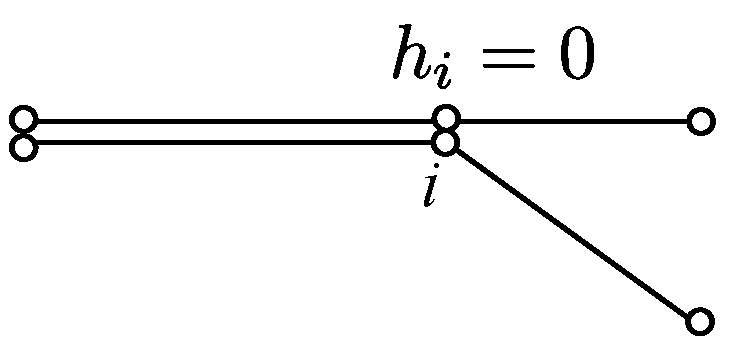
\includegraphics[scale=0.5]{graphics/masslumping.pdf}
\end{center}
\caption{Sketch of a configuration where mass-lumping would lead to an
incompatibility between the pseudo wave equation and the calculation
of $\Delta zw^{C*}$ without a specific treatment of the terms $\int\nolimits_{\Omega}\Psi_{i}~d\Omega$ in the equations.}\label{fig:masslumping}
\end{figure}

\begin{CommentBlock}{Remark:}
This corresponds to the calculation of \texttt{VOLU} with the formula
\texttt{MASBAS 2} in the subroutine \texttt{vc00pp.f}.
\end{CommentBlock}

\subsection{Suppressing wiggles: compatibility of the free surface gradient}

In the equation \eqref{eq:uc} used to calculate $\vec{u}^{aux}$,
the explicit free surface gradient is a linear function taken as:
\begin{equation}
\Grad\eta^{n}_{linear}\simeq\dfrac{{\displaystyle\int_{\Omega}}
\Grad\eta^{n}\Psi_{i}~d\Omega}{{\displaystyle\int_{\Omega}}
\Psi_{i}~d\Omega}
\end{equation}
for every degree of freedom $i$ with test function $\Psi_{i}$. This is the
"compatible" way of computing the gradient. Oscillations of $\eta$ are
not "seen" by this way of discretising the gradient and do not
trigger a velocity that would
cause artificial maxima of free-surface elevation to smooth out.
To damp such spurious oscillations, $\Grad\eta^{n}$ should be considered as a
piece-wise constant function, in a way consistant with the fact
that $\eta^{n}$ is a linear function. This is the "non compatible way"
of computing the gradient.

%However, oscillations of $\eta$ are not "seen" by this way of
%discretising the gradient and do not trigger a velocity that would
%cause artificial maxima of free-surface elevation to smooth out.
%To damp such spurious oscillations, $\Grad\eta^{n}$ should be considered as a
%piece-wise constant function, in a way consistant with the fact
%that $\eta^{n}$ is a linear function. This is the "non compatible way"
%of computing the gradient.
%In the wave equation routine of TELEMAC-3D,
%it happens that $\eta$ is written as:
%\begin{equation}
%\eta=\eta^{n}+\theta_{h}(h^{n+1}-h^{n})
%\end{equation}
%If we look at the equation \ref{contiwave} we see that the increment of depth is
On the other hand, the terms involving $\Grad(h^{n+1}-h^{n})$ in
\eqref{contiwave} are
piece-wise constant functions, since they are the gradients of a piece-wise
linear function. This is the ``non-compatible'' way of discretising the
free-surface gradient.
%These two manners to discretise the water depth are called the ``compatible''
%and ``non compatible'' discretisations.
The ``compatible'' way of discretising $\Grad\eta^n$
makes it possible to obtain a velocity field such as
\mbox{$\partial h/\partial t+\Div(h\vec{u})=0$} is fulfilled.
However, with this discretisation, oscillations of $\eta$ are invisible
because they do not trigger a velocity that would
cause artificial maxima of free-surface elevation to smooth out.
The ``non-compatible'' way of discretising $\eta$ helps
smoothing out spurious oscillations but the velocity field
does not exactly obey the continuity equation anymore.\\
%To damp such spurious oscillations, $\Grad\eta^{n}$ can be considered as a
%piece-wise constant function, in a way consistant with the fact
%that $\eta^{n}$ is a linear function. This is the "non compatible way"
%of computing the gradient.
%treated in a non compatible way because it ends up in the term:
%\begin{equation}
%\int_{\Omega_{2D}}\nu_{wave}\Grad(h^{n+1}-h^{n})\cdot\Grad\Psi_{i}^{h}d\Omega_{2D}
%\end{equation}
%where $\Grad(h^{n+1}-h^{n})$ is naturally taken as a
%piece-wise constant function, whereas the explicit part $\eta^{n}$ is
%treated in a compatible way to give $\vec{u}^{aux}$ through the equation
%\eqref{UAUX}.

To sum up, a totally compatible $\Grad\eta$ ensures
a better compatibility of the continuity equation with the velocity field,
%in the sense that we would be
%able to show a velocity $\vec{u}$ so as
%\mbox{$\dfrac{\partial h}{\partial t}+\Div(h\vec{u})=0$}.
while a totally non compatible $\Grad\eta$ makes it
possible to suppress spurious oscillations of the free-surface elevation.
It happens that the non compatible treatment of $\Grad(h^{n+1}-h^{n})$ is
not always sufficient to suppress spurious oscillations, hence the
idea of treating also the term $\Grad \eta^{n}$ in a non-compatible way.
This can be achieved by suppressing $\Grad \eta^{n}$ in the computation
of $\vec{u}^{aux}$ (equation \eqref{UAUX}), and adding the following term to
the right hand side of the continuity equation:
\begin{equation}
-\int_{\Omega_{2D}}\dfrac{\nu_{wave}}{\theta_{h}}\left[\Grad\eta^{n}\right]_{piece-wise~const.}\cdot\Grad\Psi_{i}^{h}~d\Omega_{2D}
\end{equation}
Suppressing $\Grad\eta^{n}$ in the computation of $\vec{u}^{aux}$
is actually equivalent to adding:
\begin{equation}
-\int_{\Omega}\dfrac{\nu_{wave}}{\theta_{h}}\left[\Grad\eta^{n}\right]_{linear}
\cdot\Grad\Psi_{i}^{h}~d\Omega
\end{equation}
to the right-hand side of the continuity equation. The two terms do not sum to
zero because $\Grad\eta^{n}$ is not discretised in the same
way. With a parameter $\theta^{comp}$ varying from 0 to
1 we can skip from compatible to non compatible $\Grad\eta^{n}$.
%\textcolor{red}{The figure \ref{figure1} shows the effect of a choice of
%$\theta^{comp}$=0.9 in the case of a flow around bridge piers. Wiggles are
%clearly suppressed.}
When recovering the final velocity with the formula
\eqref{eq:ucfinal}, one must not forget that $\vec{u}^{aux}$ lacks
the non compatible part of the free surface gradient, hence this lacking part
must be added, and it can only be done in a compatible way to get a
linear contribution.\\

\begin{CommentBlock}{Remark:}
When $\Grad\eta^{n}$ is referred to in the formulae, care must
be taken that in the case of tidal flats with treatment by option 1
(correction of the free surface), the function $\eta^{n}$ is piece-wise linear
and must be stored in a specific array. BIEF subroutines must be written in
order to deal with such a discretisation.
\end{CommentBlock}


\section{Space discretisation of the pressure step}

We recall that in this step the following equations are solved:
\begin{equation}
  \left\{\begin{array}{l}
    \Lap p_d^{n+1} = \dfrac{\rho}{\delta t}\Div \tilde{\vec{u}}^{n+1} \medskip \\
    \dfrac{\vec{u}^{n+1}-\tilde{\vec{u}}^{n+1}}{\delta t} = -\dfrac{1}{\rho}\Grad p_d^{n+1}
  \end{array}\right.\label{eq:pressurestepdiscrete}
\end{equation}
where $\tilde{\vec{u}}^{n+1}$ denotes the non divergence-free vector of components
$(u^C, v^C, w^D)$ (see the chapter \ref{Chapter3}).
The variational formulation is written as:%
\begin{equation}
\int_{\Omega}\Div\left(\dfrac{\delta t}{\rho}\Grad p_{d}\right)\Psi_{i}~d\Omega =
\int_{\Omega} \Div\vec{\widetilde{u}}^{n+1}\Psi_{i}~d\Omega
\end{equation}
The left-hand side of this equation is integrated by parts:
\begin{equation}
\int_{\Gamma}\Psi_{i}\dfrac{\delta t}{\rho}\Grad p_{d}\cdot \vec{n}~d\Gamma
-\int_{\Omega}\dfrac{\delta t}{\rho}\Grad p_{d}\cdot\Grad \Psi_{i}~d\Omega
=\int_{\Omega}\Div\vec{\widetilde{u}}^{n+1}\Psi_{i}\,d\Omega
\end{equation}
which is also:%
\begin{equation}
\int_{\Omega}\dfrac{\delta t}{\rho}\Grad p_{d}\cdot \Grad\Psi_{i}~d\Omega =
\int_{\Gamma}\Psi_{i}\dfrac{\delta t}{\rho}\Grad p_{d} \cdot \vec{n}~d\Gamma
-\int_{\Omega}\Div\vec{\widetilde{u}}^{n+1}\Psi_{i}~d\Omega\label{basic}%
\end{equation}


and by admitting the condition $\partial p_{d}/\partial n=0$
as a wall boundary condition for $p_{d}$, we arrive at the system:%
\begin{equation}
\int_{\Omega}\dfrac{\delta t}{\rho}\Grad p_{d}^{n+1}\cdot\Grad\Psi_{i}~d\Omega =
-\int_{\Omega}\Div\vec{\widetilde{u}}^{n+1}\Psi_{i}~d\Omega\label{lapla}
\end{equation}
This is the Poisson equation. The matrix of this system is a diffusion-type
matrix built with 1 in the place of viscosity, the pressure found being in
fact $(\delta t/\rho)p_{d}$. The boundary condition on the free surface
is $p_{d}=0$.
%This is one of the reasons why the divergence of the velocity is
%not zero after the projection (equation \ref{lapla}\ is locally cancelled by
%the Dirichlet treatment).
Once $p_{d}^{n+1}$ is known, $\vec{u}^{n+1}$ is retrieved with the second line of
\eqref{eq:pressurestepdiscrete}, which is also subjected to a variational formulation:%
\begin{equation}
\displaystyle{\int_{\Omega}}\vec{u}^{n+1}\Psi_i~d\Omega
-\displaystyle{\int_{\Omega}}\vec{\widetilde{u}}^{n+1}\Psi_i~d\Omega=
-\dfrac{\delta t}{\rho}\displaystyle{\int_{\Omega}}\Grad p_{d}^{n+1}\Psi_{i}~d\Omega
\label{projec2}%
\end{equation}
which is discretised into:
\begin{equation}
\displaystyle{\int_{\Omega}}\vec{u}_j^{n+1}\Psi_j\Psi_i~d\Omega
-\displaystyle{\int_{\Omega}}\vec{\tilde{u}}_j^{n+1}\Psi_j\Psi_i~d\Omega=
-\dfrac{\delta t}{\rho}\displaystyle{\int_{\Omega}}
p_{dj}^{n+1}\Grad\Psi_{j}\Psi_i~d\Omega
\end{equation}
for all degrees of freedom $i$, $j$. In this equation, the pressure gradient
was discretised through:
\begin{equation}
\Grad p_{d}^{n+1}=\sum_j p_{dj}^{n+1}\Grad\Psi_{j}
\end{equation}
by deriving the discretised pressure, $p(x,y,z)=\sum_jp_j\Psi_j(x,y,z)$.
The two terms of the left-hand side are mass-lumped in TELEMAC-3D (there is no
option available yet to solve the full linear system), so that the velocity
$\vec{u}^{n+1}$ is calculated through:
\begin{equation}
\vec{u}_j^{n+1}=\vec{\tilde{u}}_j^{n+1}-\dfrac{\delta t}{\rho}
\dfrac{\displaystyle{\int_{\Omega}}p_{dj}^{n+1}\Grad\Psi_{j}\Psi_i~d\Omega}
{\displaystyle{\int_{\Omega}}\Psi_{j}~d\Omega}
\end{equation}
%This projection method is the weak point of the non-hydrostatic option. The
%detailed reasons and various possible improvements were pondered in reference
%\cite{release57}.
for all degrees of freedom $i$, $j$. The term $\displaystyle{\int_{\Omega}}
\Psi_{j}~d\Omega$ in the denominator of the right-hand side is calculated in
agreement with the choice of mass-lumping on the water-height term in the
wave equation: if mass-lumping was activated, it is calculated through the
equation \eqref{eq:volu}.

\section{\label{calcul de w}Computing the conservative vertical velocity}

The conservative vertical velocity $w^C$ is calculated on the basis of the
mass conservation equation.
%As pressure is assumed hydrostatic, $w$ is required only for the
%advection step at the next time step.
As the advection is executed in the fixed transformed mesh, it is actually
$w^{C\ast}$ that we ought to know. Indeed, $w^{C}$ is only used during the calculation
of the advection terms.

\begin{CommentBlock}{Remark:}
All the demonstrations of conservation of mass for the distributive
schemes were done considering that both the advection and the mass conservation equation
(both in the form of the wave equation and in its classical form to retrieve $w^C$),
are solved in the transformed mesh. They could be solved in the fixed mesh but
this would increase the complexity of the algorithm.
\end{CommentBlock}

%It is more judicious to solve the 3D mass conservation equation in a fixed mesh.
%Thus we avoid the to and fro movement between the real and fixed mesh which makes the
%calculation unwieldy.
In fact, except in the case of advection by the method of characteristics,
where $w^{C\ast}$ is really used, it is the $\Delta zw^{C\ast}$ grouping which
appears often and which is homogeneous to a velocity (we recall that $\Delta
z$ is the depth between two planes, see the section \ref{transformation sigma}).
The formula for passing from $w^{\ast}$ to $w$, i.e. $w=\Delta zw^{C\ast}$ +
other terms (see the equation \ref{WWSTAR} below, we treat here the generalized
sigma transform case), shows that $\Delta zw^{C\ast}$ should have the same
discretization as $w^C$. It appears that in the fixed mesh, the real unknown
should be $\Delta zw^{C\ast}$ and not $w^{C\ast}$. We shall now examine a method
for calculating $\Delta zw^{C\ast}$, then how $w^C$ is found on the basis of
$\Delta zw^{C\ast}$. We first have to establish the form of the continuity
equation in the transformed mesh.

\subsection{\label{continuitytransformed}Discretisation of the continuity equation}

We recall here the continuity equation $div(\vec{u}^C)=0$ written in
the transformed mesh (equation \ref{divutransf}):
\begin{equation}
\dfrac{1}{\Delta z}\left[  \dfrac{\partial\Delta z}{\partial t}+\left(
\dfrac{\partial\left(  \Delta zu^C\right)  }{\partial x}\right)  _{y,z^{\ast}%
,t}+\left(  \dfrac{\partial\left(  \Delta zv^C\right)  }{\partial y}\right)
_{x,z^{\ast},t}+\left(  \dfrac{\partial\Delta zw^{C\ast}}{\partial z^{\ast}%
}\right)  _{x,y,t}\right]=0 \label{continuiteparplan}
\end{equation}

For each degree of freedom $i$ we should thus solve:
\begin{equation}
\int_{\Omega^{\ast}}\left[  \dfrac{\partial\Delta z}{\partial t}+\left(
\dfrac{\partial\Delta zu^C}{\partial x}\right)  _{y,z^{\ast},t}+\left(
\dfrac{\partial\Delta zv^C}{\partial y}\right)  _{x,z^{\ast},t}+\left(
\dfrac{\partial\Delta zw^{C\ast}}{\partial z^{\ast}}\right)  _{x,y,t}\right]
\Psi_{i}^{\ast}\,d\Omega^{\ast}=0
\end{equation}

With a simple sigma transformation, we would in fact get:
\begin{equation}
\int_{\Omega^{\ast}}\left[\left(\dfrac{\partial h}{\partial t}\right)
_{x,y}+\left(\dfrac{\partial hu^C}{\partial x}\right)_{y,z^{\ast},t}+\left(
\dfrac{\partial hv^C}{\partial y}\right)_{x,z^{\ast},t}+\left(  \dfrac{\partial
hw^{C\ast}}{\partial z^{\ast}}\right)_{x,y,t}\right]  \Psi_{i}^{\ast
}~d\Omega^{\ast}=0
\end{equation}
where we see the underlying depth-integrated continuity equation.
It is actually this form of the mass conservation equation that is found while
demonstrating the mass conservation of the scalar (see the section
\ref{masse traceur}). Discretized as such, this equation whose unknown is
$w^{C\ast}$ or rather $\Delta zw^{C\ast}$ leads to a system that is
ill-conditioned. The boundary conditions are
$w^{C\ast}=0$ at the bed and the free surface, if they are impermeable. The term:%
\begin{equation}
\int_{\Omega^{\ast}}\left(  \dfrac{\partial\Delta zw^{C\ast}}{\partial z^{\ast}}\right)_{x,y,t}
\Psi_{i}^{\ast}~d\Omega^{\ast}%
\end{equation}
with the unknown $\Delta zw^{C\ast}$ leads to a matrix $A$ with general term:%
\begin{equation}
A_{ij}=\int_{\Omega^{\ast}}\dfrac{\partial\Psi_{j}^{\ast}}{\partial z^{\ast}%
}\Psi_{i}^{\ast}~d\Omega^{\ast}%
\end{equation}

Outside the boundaries, the diagonal terms of this matrix are zero and it is not
invertible. From the boundary conditions at the bed and the free surface, we arrive at
disconnected solutions between two successive planes (parasitic oscillations),
or an impossibility.
%This is because the only unknown retained for solving
%mass conservation is the vertical velocity. The figure \ref{probleme surcontraint}
%shows the case of a mesh reduced to two planes, where no degree of freedom is
%available on the vertical of a point $i$ to find a vertical velocity for re-establishing
%a divergence-free flow.%
%
%\begin{figure}[tbh]%
%\centering
%\includegraphics[scale=0.5]{graphics/fluxes_overconstrained.pdf}%
%\caption{Example of a forced problem.}%
%\label{probleme surcontraint}%
%\end{figure}
%
%A vertical velocity defined on a staggered mesh would be necessary, as in
%the figure \ref{vitesse verticale}.%
%\begin{figure}[tbh]%
%\centering
%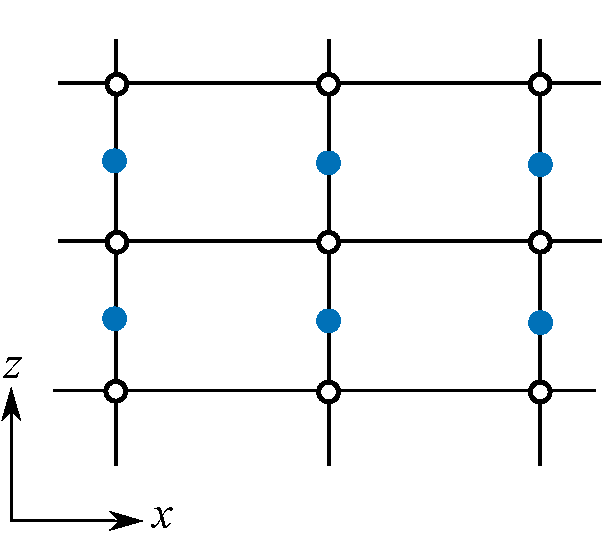
\includegraphics[scale=0.5]{graphics/fluxes.pdf}%
%\caption{Definition of a vertical velocity defined on a staggered mesh.}%
%\label{vitesse verticale}%
%\end{figure}
To circumvent this problem, a solution consists of changing unknowns or, to
be more precise, of giving a specific definition of the unknown $\Delta
zw^{C\ast}$. This definition, which will be given in the next paragraph, has
been inspired by the necessity to get an exact mass conservation of scalars
with distributive schemes. As a matter of fact, it will in due course appear
that this definition of $\Delta zw^{C\ast}$ is entirely compatible with these
distributive schemes.

\subsection{\label{wstarmoyen}Calculation of $\ \Delta zw^{C\ast}$:}

For each point $i$ of the mesh, the calculation of $\Delta zw^{C\ast}$ is done by solving:%
\begin{equation}
\int_{\Omega^{\ast}}\left(\Delta z^{n+1}-\Delta z^{n}\right)\Psi_{i}^{\ast}~d\Omega^{\ast}=
\delta t\int_{\Omega^{\ast}}\Delta z\vec{u}^C\cdot\Grad\Psi_{i}^{\ast}~d\Omega^{\ast}
-\delta t\int_{\Gamma^{\ast}}\Delta z\vec{u}^C\cdot\vec{n}\Psi_{i}^{\ast}~d\Gamma^{\ast}
\end{equation}
In the right-hand side, no time discretization of $\Delta z$ is specified yet.
Actually, it must be consistent with the 2D continuity equation, as will be
explained later, which generally imposes that $\Delta z$ is taken at time
$t^{n}$. We shall now show that the problem is well-posed if we consider that the
unknowns are the average of $\Delta zw^{C\ast}$ along the vertical of each prism.
This corresponds to a definition of the vertical velocity on a staggered mesh,
as represented in the figure \ref{vitesse verticale}.
\begin{figure}[tbh]%
\centering
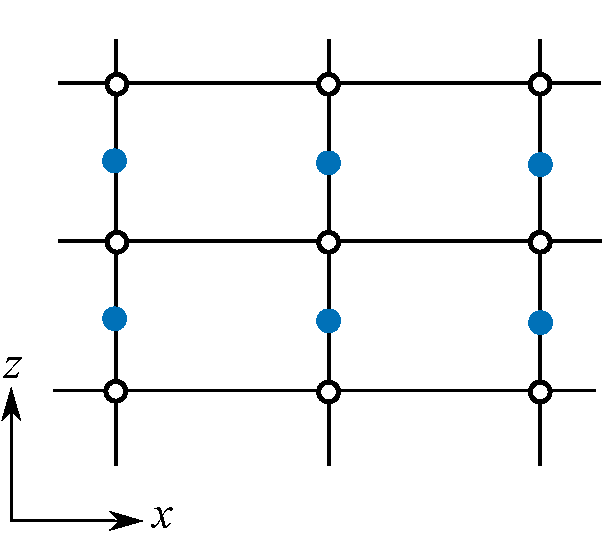
\includegraphics[scale=0.5]{graphics/fluxes.pdf}%
\caption{Definition of a vertical velocity on a staggered mesh: the blue dots represent
the degrees of freedom for the vertical velocity and the white dots represent the degrees
of freedom for the horizontal velocity.}%
\label{vitesse verticale}%
\end{figure}
Let us separate the horizontal and vertical gradients in the continuity
equation:
\begin{equation}
\begin{array}{ll}
\displaystyle{\int_{\Omega^{\ast}}}\Delta zw^{C\ast}\dfrac{\partial\Psi_{i}^{\ast}}{\partial
z^{\ast}}~d\Omega^{\ast} & =\dfrac{1}{\delta t}\displaystyle{\int_{\Omega^{\ast}}}\left(  \Delta
z^{n+1}-\Delta z^{n}\right)  \Psi_{i}^{\ast}~d\Omega^{\ast} \bigskip\\
& -\displaystyle{\int_{\Omega^{\ast}}}\Delta z\vec{u}^C\cdot\Grad_{2D}\Psi_{i}^{\ast}~d\Omega^{\ast}
+\displaystyle{\int_{\Gamma^{\ast}}}\Delta z\vec{u}^C\cdot\vec{n}\Psi_{i}^{\ast}~d\Gamma^{\ast}
\end{array}\label{CONT3D}
\end{equation}

In this form, the right-hand side only contains known terms (assuming that the
flux boundary conditions are given at the boundaries). So, we concentrate on
the left-hand side which contains unknowns. For this, it should be considered
that we work with prisms in the transformed fixed mesh, hence with horizontal
base and top. In these conditions, prisms are homothetic to the reference
prism and the 3D bases are products of one function of $x$ and $y$ and one
function of $z$ %(let us recall that for example $\Psi_{1}=(1-\alpha -\beta)\dfrac{(1-\gamma)}{2})$).
The function of $x$ and $y$ is the same as
the basis functions of triangles with linear interpolation. This makes it possible to
break down each basis as $\Psi_{i}^{\ast}=\Psi_{i}^{h}\Psi_{i}^{v}$ where $\Psi
_{i}^{h}$ only depends on $x$ and $y$, while $\Psi_{i}^{v}$ only depends on
$z$. Thus:%

\begin{equation}
\dfrac{\partial\Psi_{i}^{\ast}}{\partial z^{\ast}}=\Psi_{i}^{h}\dfrac
{\partial\Psi_{i}^{v}}{\partial z^{\ast}}%
\end{equation}

For any elevation $z^*$, we discretize the function $\Delta z\vec{u}^{C\ast}$ on the 2D domain as follows:%
\begin{equation}
\Delta z\vec{u}^{C\ast}=\sum\limits_{j=1}^{npoin2}\left[
\Delta z\vec{u}^{C\ast}(z^{\ast})\right]_{j}\Psi_{j}^{h}(x,y)
\end{equation}
where $npoin2$ is the number of degrees of freedom in the 2D mesh.

\begin{WarningBlock}{Remark:}
This choice is very impacting and constitutes a decorrelation of
the layers with regards to the vertical velocity.
%It comes to considering that the values of $\Delta z w^{C\ast}$ on each layer
%only depend on the values of the horizontal velocity above and below.
\end{WarningBlock}

%\textcolor{red}{$\Delta zw^{C\ast}(z^{\ast})$ is a function defined between 0 and 1 for each vertical line of nodes of the transformed mesh.}
The left-hand side of the equation \ref{CONT3D} then becomes:%
\begin{equation}
\sum_{j=1}^{npoin2}\left(\int_{\Omega_{2D}}\Psi_{i}^{h}\Psi_{j}^{h}~d\Omega_{2D}
\int_{0}^{1}\left[\Delta zw^{\ast}(z^{\ast})\right]_{j}\dfrac{\partial\Psi_{i}^{v}}
{\partial z^{\ast}}~dz^{\ast}\right)
\end{equation}
The mass matrix of the 2D mesh appears in $\int_{\Omega_{2D}}\Psi_{i}^{h}\Psi_{j}^{h}~d\Omega_{2D}$.
According to the position of the point $i$, the value of $\partial
\Psi_{i}^{v}/\partial z^{\ast}$ in a prism is equal to $\pm 1/\Delta z^{\ast}$,
where $\Delta z^{\ast}$ is the height of the prism (these bases
are linear; their value is 1 at the top and 0 at the bed or vice versa).

For a basis located on the plane $ip$, a plane different from the bed and
the free surface, we get:
\begin{equation}
\begin{array}{ll}
\displaystyle{\int_{0}^{1}}\left[  \Delta zw^{C\ast}(z^{\ast})\right]_{j}
\dfrac{\partial\Psi_{i}^{v}}{\partial z^{\ast}}~dz^{\ast}& =
\dfrac{1}{z_{ip}^{\ast}-z_{ip-1}^{\ast}}\displaystyle{\int_{z_{ip-1}^{\ast}}}^{z_{ip}^{\ast}}
\left[  \Delta zw^{C\ast}(z^{\ast})\right]_{j}~dz^{\ast}\\\bigskip
& -\dfrac{1}{z_{ip+1}^{\ast}-z_{ip}^{\ast}}\displaystyle{\int_{z_{ip}^{\ast}
}^{z_{ip+1}^{\ast}}}\left[  \Delta zw^{C\ast}(z^{\ast})\right]_{j}~dz^{\ast}
\end{array}
\end{equation}
The quantities retrieved here are the ones which help to calculate the
coefficients of distributive schemes (see the section
\ref{schema murd en dimension 3}).
Let us define:%
\begin{equation}
\overline{\left(  \Delta zw^{C\ast}\right)  }_{ip-\dfrac{1}{2}}^{j}=\dfrac
{1}{(z_{ip}^{\ast}-z_{ip-1}^{\ast})}\int\nolimits_{z_{ip-1}^{\ast}}%
^{z_{ip}^{\ast}}\left[  \Delta zw^{C\ast}(z^{\ast})\right]_{j}~dz^{\ast}%
\end{equation}
we finally get:%
\begin{equation}
\int\nolimits_{0}^{1}\left[\Delta zw^{C\ast}(z^{\ast})\right]_{j}
\dfrac{\partial\Psi_{i}^{v}}{\partial z^{\ast}}~dz^{\ast}=\overline{\left(
\Delta zw^{C\ast}\right)}_{ip-1/2}^{j}-\overline{\left(\Delta
zw^{C\ast}\right)}_{ip+1/2}^{j}%
\end{equation}

For a point located on the bed, we have:%
\begin{equation}
\int_{0}^{1}\,\left[  \Delta zw^{C\ast}(z^{\ast})\right]  _{j}%
\dfrac{\partial\Psi_{i}^{v}}{\partial z^{\ast}}~dz^{\ast}=+\overline{\left(
\Delta zw^{C\ast}\right)  }_{1+1/2}^{j}%
\end{equation}
and at the surface:%
\begin{equation}
\int_{0}^{1}\,\left[  \Delta zw^{C\ast}(z^{\ast})\right]  _{j}%
\dfrac{\partial\Psi_{i}^{v}}{\partial z^{\ast}}~dz^{\ast}=-\overline{\left(
\Delta zw^{C\ast}\right)  }_{np-1/2}^{j}%
\end{equation}

We arrive at a series of linear systems (one per plane),
which, after discretisation, read:%
\begin{equation}
\begin{array}{l}
\displaystyle{\sum_{j=1}^{npoin2}}\left(
\int_{\Omega_{2D}}\Psi_{i}^{h}\Psi_{j}^{h}~d\Omega_{2D}\left[
\overline{\left(\Delta zw^{C\ast}\right)}_{ip+1/2}^{j}
-\overline{\left(\Delta zw^{C\ast}\right)}_{ip-1/2}^{j}
\right]\right) = \\\bigskip
-\dfrac{1}{\delta t}\displaystyle{\int_{\Omega^{\ast}}}
\displaystyle{\sum_{j=1}^{npoin3}}
\left(\Delta z_j^{n+1}-\Delta z_j^{n}\right)
\Psi_{j}^{\ast}\Psi_{i}^{\ast}~d\Omega^{\ast}
+\int_{\Omega^{\ast}}\displaystyle{\sum_{j=1}^{npoin2}}\Delta z_j\Psi_{j}^{\ast}\displaystyle{\sum_{k=1}^{npoin2}}\Psi_{k}^{\ast}\vec{u}_k^C\cdot\Grad_{2D}\Psi_{i}^{\ast}~d\Omega^{\ast}\\\bigskip
-\displaystyle{\int_{\Gamma_{liq}^{\ast}}}\displaystyle{\sum_{j=1}^{npoin2}}\Delta z_j\Psi_{j}^{\ast}\displaystyle{\sum_{k=1}^{npoin2}}\vec{u}_k^C\Psi_{k}^{\ast}\cdot\vec{n}\Psi_{i}^{\ast}~d\Gamma^{\ast}
\end{array}\label{tridw2}
\end{equation}
We deliberately kept the summation signs in the equations because they
either run on the 2D points or on the 3D points.
%
%\begin{WarningBlock}{Warning:}
%Is this well posed?
%\end{WarningBlock}
%
In this form, the
new unknowns $\overline{\left(\Delta zw^{C\ast}\right)  }_{ip+1/2}^{j}$
can be found layer by layer starting from the bed, or in the same
way from the surface.
The system's matrix is always the same mass matrix and is easily invertible.
On the other hand, there are still too many equations and it is likely that, if
we start from the bed, the boundary condition at the free surface will not
be retrieved. This does not happen since the depth-integrated
continuity equation was resolved in a compatible way to calculate the
free surface. In fact, the sum of all
equations, layer after layer, eliminates all the unknowns $\overline{\left(
\Delta zw^{C\ast}\right)  }_{ip+1/2}^{j}$ and restores the mass
conservation expression of the pseudo-wave equation.
If the latter has been correctly resolved, the linear system
of the last plane is deduced from the others,
and hence it cannot give rise to contradictions.\\

The equation \ref{tridw2}
is actually simplified by mass lumping.
In this case, the left-hand side reads:
\begin{equation}
\displaystyle{\sum_{j=1}^{npoin2}}\left(\int_{\Omega_{2D}}\Psi_{i}^{h}\Psi_{j}^{h}~d\Omega_{2D}\right)
\left[  \overline{\left(\Delta zw^{C\ast}\right)  }_{ip+1/2}^{i}-\overline{\left(  \Delta
zw^{C\ast}\right)  }_{ip-1/2}^{i}\right]
\end{equation}
and the system is solved by a mere division of the right-hand side by
$\int\nolimits_{\Omega_{2D}}\Psi_{i}^{h}~d\Omega_{2D}$. The same mass lumping
must also be done when computing the corresponding terms in the scalar
equation (see the section \ref{murdconservation} and the computation of the terms $b_{i}$) in order to ensure the mass conservation.


%%%%%%%%%%%%%%%%%%%%%%%%%%%%%%%%%%%%%%%%%%%%%%%%%%%%%%%%%%%%%%
%%%%%%%%%%%%%%%%%%%%%%%%%%%%%%%%%%%%%%%%%%%%%%%%%%%%%%%%%%%%%%
%%%%%%%%%%%%%%%%%%%%%%%%%%%%%%%%%%%%%%%%%%%%%%%%%%%%%%%%%%%%%%



\subsection{Nodal values of $w^{C\ast}$}

One would now expect that we deduce $w^{C\ast}$ from $\Delta zw^{C\ast}$ by
dividing by $\Delta z$. This is not a good idea. As a matter of fact we need
nodal values of $w^{C\ast}$, e.g. for the advection in the transformed mesh
with the method of characteristics, but if we write $w^C$ in the transformed
mesh, we get:%

\begin{equation}
w^C=\dfrac{dz}{dt}=\dfrac{\partial z}{\partial t}+u^C\dfrac{\partial z}{\partial
x}+v^C\dfrac{\partial z}{\partial y}+w^{C\ast}\dfrac{\partial z}{\partial z^{\ast}}%
\end{equation}
and so we have:%

\begin{equation}
\Delta zw^{C\ast}=\,-\dfrac{\partial z}{\partial t}-u^C\dfrac{\partial z}{\partial
x}-v^C\dfrac{\partial z}{\partial y}+w^C \label{Wintransformedmesh}%
\end{equation}

We can deduce from this latter equation that if $w^C$ is a linear function, then
$\Delta zw^{C\ast}$ is also a linear function. To get this linear function, we
need to have nodal values of $\Delta zw^{C\ast}$, which can be obtained by the
following formula using the layer-averaged values of the previous paragraph:%
\begin{equation}
\overline{\left(  \Delta zw^{C\ast}\right)  }_{ip}^{j}=\dfrac{\overline{\left(
\Delta zw^{C\ast}\right)  }_{ip-1/2}^{j}+\overline{\left(\Delta
zw^{C\ast}\right)}_{ip+1/2}^{j}}{2}%
\end{equation}
At the boundaries, i.e. at the bed and at the free surface, we know that
the impermeability condition imposes that $\Delta zw^{C\ast}=0$. We now have a
linear function $\Delta zw^{C\ast}$. When computing the characteristics in the
transformed mesh, the vertical velocity in a layer will be this linear
function $\Delta zw^{C\ast}$ divided by $\Delta z$ which is locally a function
of $x$ and $y$.

\subsection{\label{wwstar}Passing from $\Delta zw^{C\ast}$ to $w^C$ -- only for the hydrostatic option}

As the advection is done in the transformed mesh, $w^C$ is actually never used,
but users generally expect to see it in the results, and so it must be built
when the hydrostatic option is used because the momentum equation along $z$
is not solved. This is done with the equation \ref{Wintransformedmesh},
which is discretized in time in the form:%
\begin{equation}
w^{Cn+1}=(\Delta zw^{C\ast})^{n+1}+\dfrac{z^{n+1}-z^{n}}{\delta t}+u^C\dfrac
{\partial z^{n}}{\partial x}+v^C\dfrac{\partial z^{n}}{\partial y} \label{WWSTAR}%
\end{equation}
This equation is integrated layer by layer over the vertical in the
transformed mesh, and then multiplied by a test function and integrated on the
2D mesh. It gives:%
\begin{equation}
\begin{array}{ll}
\displaystyle{\int_{\Omega_{2D}}}\left(\int_{z_{ip}^{\ast}}^{z_{ip+1}^{\ast}}
w^{Cn+1}~dz^{\ast}\right)  \Psi_{i}^{h}d\Omega_{2D} & =\displaystyle{\int_{\Omega_{2D}}}\left(
\int_{z_{ip}^{\ast}}^{z_{ip+1}^{\ast}}\left(  \Delta zw^{C\ast}\right)
^{n+1}~dz^{\ast}\right)  \Psi_{i}^{h}d\Omega_{2D}\\\bigskip
& +\displaystyle{\int_{\Omega_{2D}}}\left(  \int_{z_{ip}^{\ast}}^{z_{ip+1}^{\ast}}\left(
\dfrac{z^{n+1}-z^{n}}{\delta t}+u^C\dfrac{\partial z^{n}}{\partial x}
+v^C\dfrac{\partial z^{n}}{\partial y}\right)  ~dz^{\ast}\right)
\Psi_{i}^{h}~d\Omega_{2D}
\end{array}
\end{equation}
where $ip$ is the number of the lower plane of the layer, and $i$ is the
global number of a node in the 2D mesh. As $w$ is linear, we have:%

\begin{equation}
\int_{z_{ip}^{\ast}}^{z_{ip+1}^{\ast}}w^{Cn+1}~dz^{\ast}=(w_{ip}^{Cn+1}%
+w_{ip+1}^{Cn+1})\dfrac{\Delta z_{ip+1/2}^{\ast}}{2}%
\end{equation}
By using similar formulae for $(z^{n+1}-z^{n})/\delta t$, we get:%
\begin{equation}
\begin{array}{ll}
\displaystyle{\int_{\Omega_{2D}}}(w_{ip}^{Cn+1}+w_{ip+1}^{Cn+1})\Psi_{i}^{h}\,d\Omega
_{2D}& =2\displaystyle{\int_{\Omega_{2D}}}(\Delta zw^{C\ast})_{ip+1/2}^{n+1}\Psi_{i}^{h}
~d\Omega_{2D}\\\bigskip
& +\dfrac{1}{\delta t}\displaystyle{\int_{\Omega_{2D}}}(z_{ip}^{n+1}+z_{ip+1}^{n+1}-z_{ip}%
^{n}-z_{ip+1}^{n})\Psi_{i}^{h}~d\Omega_{2D} \\\bigskip
& +\dfrac{2}{\Delta z_{ip+1/2}^{\ast}}\displaystyle{\int_{\Omega_{2D}}}\left(  \int%
_{z_{ip}^{\ast}}^{z_{ip+1}^{\ast}}\left(  u^C\dfrac{\partial z^{n}}{\partial
x}+v^C\dfrac{\partial z^{n}}{\partial y}\right)  ~dz^{\ast}\right)  \Psi_{i}^{h}
~d\Omega_{2D}
\end{array}
\end{equation}
We recognize here a series of linear systems on the 2D mesh, the matrix being
the mass matrix. For every layer in the mesh, we shall get $w_{ip}%
^{Cn+1}+w_{ip+1}^{Cn+1}$. If we start from $ip=1$, the first value $w_{1}^{Cn+1}$
is given by the boundary condition on the bed,
and then the boundary condition at the free surface
should be naturally ensured. Another possibility is to start from the free
surface, and going down to the bed.
Lest the truncation errors or a lack of compatibility in the discretization
should give a wrong boundary condition after going up or down, we build both
solutions, creating a series of $w_{ip}^{Cup}$ and $w_{ip}^{Cdown}$, where
$w_{1}^{Cup}$ is obtained by the boundary condition at the bed and
$w_{np}^{Cdown}$ is obtained from the boundary condition at the free surface.
The final value of the vertical velocity is then obtained by the formula:%
\begin{equation}
w_{ip}^{Cn+1}=\dfrac{(ip-1)w_{ip}^{Cdown}+(np-ip)w_{ip}^{Cup}}{np-1}%
\end{equation}
where $np$ is still the number of superimposed meshes of triangles.

\section{\label{scalar in dimension 3}Space discretisation of the scalar equation\index{scalar}}

The scalar equation \eqref{eq:scalarEquation} in a moving mesh is
recalled below:
\begin{equation}
\dfrac{\partial T}{\partial t}+\left((\vec{u}-\vec{c})\cdot\Grad\right)
T - \Div\left(K_E\Grad(T)\right)+Q=0
\end{equation}
The advection takes place in the fixed transformed mesh
with the methods presented in the section \ref{equations de transport}.
It is either coupled with the diffusion (the case of the SUPG scheme) or
solved before the diffusion (the case of the characteristics
and distributive schemes). The advection equation is written as:%
\begin{equation}
\int_{\Omega^{\ast}}\Delta z(T^{n+1}-T^{n})\Psi_{i}^{\ast}~d\Omega^{\ast}
+\delta t\int_{\Omega^{\ast}}\Delta z\vec{u}^{\ast}\cdot\Grad T
\Psi_{i}^{\ast}~d\Omega^{\ast}=0
\end{equation}

We recall that the velocity of the mesh is also taken into
account by this formula, as explained in the section \ref{sec:ALE}.
In 1995, Janin (see \cite{janin95}) found a remarkable solution for building a monotonic and at the same time conservative scheme:
\begin{itemize}
\item the use of a distributive scheme called the MURD scheme
(see the section \ref{schema murd en dimension 3});
\item the choice of advection in a mesh fixed in time $t^{n+1}$,
with $T$ written in an explicit way in the term $\Grad T$
(see the demonstration of conservation of the scalar in the
section \ref{masse traceur});
\item a compatible resolution of the mass conservation equation,
with a variable $\Delta zw^{C\ast}$ averaged per layer as seen
in the section \ref{wstarmoyen}.
\end{itemize}

Only a good comprehension of these three points allows one to
appreciate the interest and originality of this approach.
Diffusion has fewer constraints and is calculated in the real mesh.
In 2005 mass conservation of the scalar was extended to the SUPG\ advection scheme, using the same ideas.

\section{\label{masse en 3D}The conservation of mass}

\subsection{\label{masse d'eau}Conservation of mass of water%
\index{conservation of mass!Navier--Stokes}%
}

The conservation of mass on a domain $\Omega$ is written as:
\begin{equation}
{\displaystyle\int\nolimits_{\Omega}}
\left(\dfrac{\partial u}{\partial x}+\dfrac{\partial v}{\partial y}
+\dfrac{\partial w}{\partial z}\right) ~ d\Omega=0
\end{equation}
With the calculation of $\Delta zw^{C*}$ through the resolution of this
equation in the transformed mesh, we ensure that the conservative
velocity field is indeed almost divergence-free, considering
that the discretisation of the continuity equation induces some errors.
Overall conservation of mass is actually possible without a local
resolution of the continuity, hence without a divergence-free
3D velocity field. A more localized conservation will be imposed
for the conservation of the scalar.

\subsection{\label{masse traceur}Conservation of scalar
\index{conservation of mass!scalar}\index{scalar}
}

The conservation of the scalar is written as:
\begin{equation}
\int_{\Omega}(T^{n+1}-T^{n})~d\Omega+\delta t\int_{\Gamma}T\vec{u}\cdot
\vec{n}~d\Gamma-\delta t\int_{\Gamma}K_{E}\dfrac{\partial T}{\partial n}
~d\Gamma-\delta t\int_{\Omega}Q~d\Omega=0
\label{eq:conservationTraceur}
\end{equation}
where $Q$ is a source term. If Dirichlet-type boundary conditions
\index{Dirichlet boundary conditions (imposed values)}
are imposed on the boundaries, this spoils the conservation and
a correction is needed
(see below in the section \ref{dirichletdistributif}).
The non-conservative equation resolved for each degree of
freedom is as follows:
\begin{equation}
\int_{\Omega}\left(\dfrac{\partial T}{\partial t}+(\vec{u}^C-\vec{c})
\cdot\Grad T-\nabla\left(K_{E}\nabla T\right)-Q\right)\Psi_{i}~d\Omega=0
\end{equation}

Considering only the advection of the scalar we have:
\begin{equation}
\int_{\Omega}(T^{n+1}-T^{n})d\Omega+\delta t\int_{\Omega}(\vec{u}^C-\vec{c})
\cdot \Grad T ~d\Omega=0
\label{eq:advectionTraceur}
\end{equation}
which, with \eqref{eq:conservationTraceur}, is equivalent to:
\begin{equation}
\int_{\Omega}(T^{n+1}-T^{n})d\Omega+\delta t\int_{\Gamma}T\vec{u}^C\cdot
\vec{n}~d\Gamma=0
\end{equation}
We dropped the diffusion term and the creation/destruction
term $Q$ which are not really a problem for the conservation of mass.
%To achieve conservation, it would thus be necessary to add the
%following term to the right-hand side of \eqref{eq:advectionTraceur}:
%\begin{equation}
%\delta t\int_{\Omega}T\Div\vec{u}^Cd\Omega
%\end{equation}
%which, in principle, is zero. This is where a compatibility
%condition with the continuity equation appears.
This formulation in the real domain actually masks the problem of the
evolution of $\Omega$ and the fact that the advection step
of the scalar should be done in the fixed mesh if the advection
was already done there. Written in the fixed mesh,
the conservation of the scalar reads:
\begin{equation}
\int_{\Omega^{\ast}}(\Delta z^{n+1}T^{n+1}-\Delta z^{n}T^{n})d\Omega^{\ast}
+\delta t\int_{\Gamma^{\ast}}\Delta zT\vec{u}^{C\ast}\cdot\vec{n}
~d\Gamma^{\ast}=0
\end{equation}
while the advection equation of the scalar
in the fixed mesh at an instant taken between $t^{n}$ and $t^{n+1}$
gives:
\begin{equation}
\int_{\Omega^{\ast}}\Delta z(T^{n+1}-T^{n})~d\Omega^{\ast}+\delta t
\int_{\Omega^{\ast}}\Delta z\vec{u}^{\ast}\cdot\Grad T~d\Omega^{\ast}=0
\label{convT}
\end{equation}
In this equation, if the fixed mesh is chosen at instant $t^{n}+\theta
_{h}\delta t$, the following should be taken:
\begin{equation}
\Delta z=\theta_{h}\Delta z^{n+1}+(1-\theta_{h})\Delta z^{n}%
\end{equation}
We then need to choose an implicit expression of $T$ for calculating its
gradient. If we define:
\begin{equation}
T=\theta_{T}T^{n+1}+(1-\theta_{T})T^{n}%
\end{equation}
the integral equation above, by adding the following null
expression to it:
\begin{equation}
\delta t\int_{\Gamma^{\ast}}\Delta zT\vec{u}^{C\ast}\cdot\vec{n}~d\Gamma^{\ast}
-\delta t\int_{\Gamma^{\ast}}\Delta zT\vec{u}^{C\ast}\cdot\vec{n}~d\Gamma^{\ast}
\end{equation}
can then be written as:
\begin{equation}
\begin{array}{l}
\displaystyle{\int_{\Omega^{\ast}}}
(\Delta z^{n+1}T^{n+1}-\Delta z^{n}T^{n})~d\Omega^{\ast}
+\delta t\displaystyle{\int_{\Gamma^{\ast}}}
\Delta zT\vec{u}^{C\ast}\cdot\vec{n}~d\Gamma^{\ast}\bigskip\\
-\displaystyle{\int_{\Omega^{\ast}}}
\theta_{h}T^{n}(\Delta z^{n+1}-\Delta z^{n})~d\Omega^{\ast}
+(1-\theta_{T})\delta t\displaystyle{\int_{\Omega^{\ast}}}
\Delta z\vec{u}^{C\ast}\cdot\Grad T^{n}~d\Omega^{\ast}\bigskip\\
-(1-\theta_{T})\delta t\displaystyle{\int_{\Gamma^{\ast}}}
\Delta zT^{n}\vec{u}^{C\ast}\cdot\vec{n}~d\Gamma^{\ast}
-\displaystyle{\int_{\Omega^{\ast}}}
(1-\theta_{h})T^{n+1}(\Delta z^{n+1}-\Delta z^{n})~d\Omega^{\ast}\bigskip\\
+\theta_{T}\delta t\displaystyle{\int_{\Omega^{\ast}}}
\Delta z\vec{u}^{C\ast}\cdot\Grad T^{n+1}~d\Omega^{\ast}
-\theta_{T}\delta t\displaystyle{\int_{\Gamma^{\ast}}}
\Delta zT^{n+1}\vec{u}^{C\ast}\cdot\vec{n}~d\Gamma^{\ast}=0
\end{array}
\end{equation}

It has to be proved that the last three lines are zero to guarantee the
conservation of the scalar. By breaking down $T^{n}$ and $T^{n+1}$ on the
basis $\Psi_{i}^{\ast}$ of the transformed mesh,
two conditions are sufficient:
\begin{equation}
\theta_{h}+\theta_{T}=1
\end{equation}
and:
\begin{equation}
\int_{\Omega^{\ast}}(\Delta z^{n+1}-\Delta z^{n})\Psi_{i}^{\ast}~d\Omega^{\ast}
-\delta t\int_{\Omega^{\ast}}\Delta z\vec{u}^{C\ast}\cdot\Grad \Psi_{i}^{\ast}
~d\Omega^{\ast}+\delta t\int_{\Gamma^{\ast}}\Psi_{i}^{\ast}\Delta z\vec{u}^{C\ast}\cdot\vec{n}~d\Gamma^{\ast}=0
\label{eq:cond2}
\end{equation}

At this point the variational formulation of the depth-integrated mass
conservation equation appears.
We arrive at \textbf{two fundamental conclusions}:
\begin{itemize}
\item the conservation of the mass of the scalar requires a compatible
treatment of the depth-integrated continuity equation so that the condition
\eqref{eq:cond2} is satisfied;
\item the condition $\theta_{h}+\theta_{T}=1$ which signifies,
for instance, that if an explicit scheme is used to calculate
the value of $\int_{\Omega^{\ast}}\Delta z\vec{u}\cdot\Grad T~d\Omega^{\ast}$,
the advection step should be done (paradoxically) in the
mesh fixed at time $t^{n+1}$. A more detailed demonstration of scalar
conservation will be given in the section \ref{sourcesdistributive}
below, with the example of a distributive advection scheme.
\end{itemize}

\section{\label{sources3d}Sources and sinks of fluid in the Navier--Stokes equations\index{sources}\index{sinks}}

In order to deal with water or scalar inputs into a domain, \textit{e.g.} drainage pipes whose dimensions are less than the size of finite elements, we use the concept of sources and sink points in the domain.
The fluid flow, with or without scalar, is considered as entering
the calculation domain at a single point.
%This concept, already treated for the Saint-Venant equations, is artificial in certain aspects and for the Navier--Stokes equations requires a thorough examination.

\subsection{\label{sourcesoffluid}Sources of fluid}

In 3D, it is now the continuity equation $\Div \vec{u}=0$ which is
no longer verified locally. In the transformed mesh, starting again from
the equation \ref{divutransf}, we now have to solve:%

\begin{equation}
\int_{\Omega^{\ast}}\left[\left(\dfrac{\partial\Delta z}{\partial t}\right)_{x,y}
+\left(\dfrac{\partial\Delta zu^C}{\partial x}\right)_{y,z^{\ast},t}
+\left(\dfrac{\partial\Delta zv^C}{\partial y}\right)_{x,z^{\ast},t}
+\left(\dfrac{\partial\Delta zw^{C\ast}}{\partial z^{\ast}}\right)_{x,y,t}\right]
\Psi_{i}^{\ast}~d\Omega^{\ast}
=\int_{\Omega^{\ast}}\Delta z\Div\vec{u}^{C\ast}\Psi_{i}^{\ast}~d\Omega^{\ast}
\end{equation}
Recall that \mbox{$\int_{\Omega^{\ast}}\Delta z\Div\vec{u}^C\Psi_{i}^{\ast}~d\Omega^{\ast}=\int_{\Omega}\Div\vec{u}\Psi_{i}~d\Omega$}. With inputs our
outputs of fluid in the domain, $\Div\vec{u}^C$ will not be
zero in certain points. The integral $\Div\vec{u}^C$ around a domain
surrounding a source point will be the discharge
of the source $Q_{sce}$.
%As in 2D, but taking into account the vertical,
To take this into account, one solution consists of
adding to the right-hand side of the continuity equation the term:%
\begin{equation}
\sum_{i3d\text{\thinspace above\thinspace\thinspace}i2d}\dfrac{
\displaystyle{\int_{\Omega}}
Q_{sce}\Psi_{isce}\Psi_{i3d}~d\Omega}{\displaystyle{\int_{\Omega}}
\Psi_{isce}~d\Omega}
\end{equation}
where $isce$ is the point where the fluid is entering or leaving.
It is worth noticing that:
\begin{equation}
\sum_{i3d\text{\thinspace above\thinspace\thinspace}i2d}
\dfrac{\displaystyle{\int_{\Omega}}
Q_{sce}\Psi_{isce}\Psi_{i3d}~d\Omega}{\displaystyle{\int_{\Omega}}
\Psi_{isce}~d\Omega}\text{ }\neq\text{ }\dfrac{
\displaystyle{\int_{\Omega_{2D}}}
Q_{sce}\Psi_{isce}^{h}\Psi_{i2d}~d\Omega_{2D}}{\displaystyle{\int_{\Omega_{2D}}}
\Psi_{isce}^{h}~d\Omega_{2D}}%
\end{equation}
On the other hand, the series of linear systems giving
the vertical velocities averaged over each plane is then
written for every point $i$ in the 2D mesh as:%
\begin{equation}
\begin{array}{l}
\displaystyle{\sum_{j=1}^{npoin2}}\left\{
\displaystyle{\int_{\Omega_{2D}}}\Psi_{i}^{h}\Psi_{j}^{h}~d\Omega_{2D}
\left[\overline{\left(\Delta zw^{C\ast}\right)}_{ip+1/2}^{j}
-\overline{\left(\Delta zw^{C\ast}\right)}_{ip-1/2}^{j}\right]
\right\}\\\bigskip
=-\dfrac{1}{\delta t}\displaystyle{\int_{\Omega^{\ast}}}
\left(\Delta z^{n+1}-\Delta z^{n}\right)
\Psi_{i}^{\ast}~d\Omega^{\ast}+\displaystyle{\int_{\Omega^{\ast}}}
\Delta z\vec{u}\cdot\Grad_{2D}\Psi_{i}^{\ast}~d\Omega^{\ast}\\\bigskip
-\displaystyle{\int_{\Gamma_{liq}^{\ast}}}
\Delta z\vec{u}\cdot\vec{n}\Psi_{i}^{\ast}~d\Gamma^{\ast}
+\displaystyle{\sum_{i3d\text{\thinspace above\thinspace\thinspace}i2d}}
\dfrac{\displaystyle{\int_{\Omega}}Q_{sce}\Psi_{isce}
\Psi_{i3d}~d\Omega}{\displaystyle{\int_{\Omega}}\Psi_{isce}~d\Omega}
\end{array}
\end{equation}
The domain $\Omega$ is here considered at the same instant as
the other flux terms.

\subsection{\label{sourcesdistributive}Sources of scalar with a distributive scheme\index{distributive scheme}}

Having seen both the conservation of scalar mass
and the sources of water, we
are now in a position to understand how to
deal with sources of scalars. As a
matter of fact it is necessary to rely on the
proof of conservation of the
scalar mass to find out which source terms to apply to it.
The treatment of the advection terms has its importance
and we take here the example of the MURD
scheme which will be presented in the section
\ref{schema murd en dimension 3}. It
is an explicit scheme and it is about the only thing to recall in what
follows. We recall the following notations:

\begin{equation}
FLUINT(i)=\int_{\Omega^{\ast}}\Delta z\vec{u}^C\cdot\Grad_{2D}\Psi_{i}^{\ast}
~d\Omega^{\ast}
\end{equation}

\begin{equation}
FLUVER(i)=\int_{\Omega^{\ast}}\Delta zw^{C\ast}\dfrac{\partial\Psi_{i}^{\ast}
}{\partial z^{\ast}}~d\Omega^{\ast}
\end{equation}

\begin{equation}
SOURCE(i)=\dfrac{\int\nolimits_{\Omega}Q_{sce}\Psi_{isce}\Psi_{i}d\Omega}
{\int_{\Omega}\Psi_{isce}~d\Omega}\alpha(i)
\end{equation}

\begin{equation}
FLUEXT(i)=\int_{\Gamma_{liq}^{\ast}}\Delta z\vec{u}^C\cdot\vec{n}
\Psi_{i}^{\ast}~d\Gamma^{\ast}
\end{equation}

\bigskip The continuity equation is then written as:
\begin{equation}
\dfrac{1}{\delta t}\int_{\Omega^{\ast}}\left(\Delta z^{n+1}-\Delta z^{n}
\right)\Psi_{i}^{\ast}~d\Omega^{\ast}=FLUINT(i)+FLUVER(i)-FLUEXT(i)+SOURCE(i)
\end{equation}


The equation for the scalar $T$ is as follows:%
\begin{equation}
\dfrac{1}{\delta t}\int_{\Omega^{\ast}}\Delta z^{n+1}
\left(T^{n+1}-T^{n}\right)  \Psi_{i}^{\ast}~d\Omega^{\ast}=
-\int_{\Omega^{\ast}}\Delta z\vec{u}\cdot\Grad T^{n}\Psi_{i}^{\ast}~d\Omega^{\ast}+SOURCE\_TRAC(i)
\end{equation}
where the term $\int_{\Omega^{\ast}}\Delta z\vec{u}%
.\Grad(T^{n})\Psi_{i}^{\ast}d\Omega^{\ast}$ is explicit and
calculated by the distributive scheme.
$SOURCE\_TRAC(i)$ is the source term we look for.
The overall conservation of the scalar mass is shown by
first multiplying all the continuity equations by
$T_{i}^{n}$, then by adding them, and eventually by adding to
them all the scalar equations, which gives:

\begin{equation}
\begin{array}{l}
\dfrac{1}{\delta t}\displaystyle{\int_{\Omega^{\ast}}}
\left(\Delta z^{n+1}-\Delta z^{n}\right)T^{n}~d\Omega^{\ast}
+\dfrac{1}{\delta t}\displaystyle{\int_{\Omega^{\ast}}}\Delta z^{n+1}
\left(T^{n+1}-T^{n}\right)  ~d\Omega^{\ast}\bigskip\\
=\displaystyle{\sum_{i}}FLUINT(i)T_{i}^{n}+
\displaystyle{\sum_{i}}FLUVER(i)T_{i}^{n}
-\displaystyle{\sum_{i}}FLUEXT(i)T_{i}^{n}\bigskip\\
+\displaystyle{\sum_{i}}SOURCE(i)T_{i}^{n}
-\displaystyle{\int_{\Omega^{\ast}}}
\Delta z\vec{u}\cdot\Grad T^{n}~d\Omega^{\ast}
+\displaystyle{\sum_{i}}SOURCE\_TRAC(i)
\end{array}
\end{equation}

Now, the distributive scheme ensures that:%
\begin{equation}
\sum\limits_{i}FLUINT(i)T_{i}^{n}+\sum\limits_{i}FLUVER(i)T_{i}^{n}%
-\int_{\Omega^{\ast}}\Delta z\vec{u}\cdot\Grad T^{n}~d\Omega^{\ast}=0
\end{equation}
because it simply performs a redistribution of the first
two terms without changing its sum. We finally arrive at:
\begin{equation}
\begin{array}{ll}
\dfrac{1}{\delta t}\displaystyle{\int_{\Omega^{\ast}}}
\left(\Delta z^{n+1}T^{n+1}-\Delta z^{n}T^{n}\right)~d\Omega^{\ast} & =
-\displaystyle{\sum_{i}}FLUEXT(i)T_{i}^{n}
+\displaystyle{\sum_{i}}SOURCE(i)T_{i}^{n}\bigskip\\
& +\displaystyle{\sum_{i}}SOURCE\_TRAC(i)
\end{array}
\end{equation}
In the case of a source with a scalar value $T_{sce}$,
the conservation of mass of scalar imposes that:
\begin{equation}
\sum_{i}SOURCE(i)T_{i}^{n}+\sum_{i}SOURCE\_TRAC(i)=Q_{sce}T_{sce}
\end{equation}
One solution for a source is then:
\begin{equation}
SOURCE\_TRAC(i)=(T_{sce}-T_{i}^{n})SOURCE(i)
\end{equation}
If there are several sources, there should be a distinction between the
$SOURCE(i)$ vectors for each source.
If the source is actually a sink, then $SOURCE(i)$
is negative and a different treatment is necessary.
As a matter of fact, in a sink, the value of the
scalar now exiting the domain is not $T_{sce}$,
but rather the local value $T_{i}$, so that $SOURCE\_TRAC(i)$
must in fact be cancelled. Everywhere $T_{sce}$ appears, it must
be replaced by $T_{i}$ (here $T_{i}^{n} $ because we have an explicit
scheme, but it could as well be $T_{i}^{n+1}$ with an implicit scheme).
To take sinks into account as well as sources, we must thus
consider that:
\begin{equation}
SOURCE\_TRAC(i)=(T_{sce}-T_{i}^{n})MAX(SOURCE(i),0)
\end{equation}


\subsection{\label{dirichletdistributif}Dirichlet boundary conditions with a
distributive scheme%
\index{Dirichlet boundary conditions (imposed values)}%
}

As the previous subsections give a full proof of the mass conservation of the
scalar, we are now in a position to deal with the problem of imposed boundary
conditions. The distributive schemes pay no attention to prescribed values at
the boundaries; they just take the scalar at time $t^{n}$ and ensure mass
conservation and monotonicity. A user may want to prescribe given values at an
entrance to the domain, or a given scalar flux. If nothing special is done the
flux of the scalar through the boundaries (here positive if entering the
domain) will be:%

\begin{equation}
observed\,\,flux=-\int\nolimits_{\Gamma_{liq}^{\ast}}\Delta zT^{n}%
\vec{u}.\vec{n}\,d\Gamma^{\ast}%
\end{equation}
%

\begin{equation}
=-\sum\limits_{i\,}T_{i}^{n}\int\nolimits_{\Gamma_{liq}^{\ast}}\Delta
z\vec{u}\cdot\vec{n}\Psi_{i}^{\ast}~d\Gamma^{\ast}=-\sum\limits_{i\,}%
T_{i}^{n}FLUEXT(i)
\end{equation}
and the imposed values will not be ensured. The summation on $i$ must be
understood as $i$ being on the boundary with prescribed values. The user would
in fact like to have:%

\begin{equation}
wanted\,\,flux=-\int\nolimits_{\Gamma_{liq}^{\ast}}\Delta zT^{imposed}%
\vec{u}\cdot\vec{n}\,d\Gamma^{\ast}\ \text{\ and }\ T_{i}^{n+1}%
=T_{i}^{imposed}\text{ on boundaries}%
\end{equation}


Both conditions are not compatible. Brutally setting $T_{i}^{n+1}%
=T_{i}^{imposed}$ or $T_{i}^{n}=T_{i}^{imposed}$ on boundaries will add or
remove scalar mass in the domain, because the basis functions on the
boundaries go inside the domain, thus creating an artificial flux. We propose
here a relaxation of the Dirichlet conditions which consists of replacing
$T_{i}^{n}$ by:%

\begin{equation}
T_{i}^{n}+\theta(T_{i}^{imposed}-T_{i}^{n})=T_{i}^{n}+\Delta T^{n}
\label{apriori}%
\end{equation}
on liquid boundaries with imposed values, with $0<\theta<1$. $\theta$ is
computed so that the sum of the \textit{a priori} added mass and\ the observed
flux gives the wanted flux. The added mass is:%

\begin{equation}
added\,\,mass=\theta(T_{i}^{imposed}-T_{i}^{n})\int_{\Omega^{\ast}}\Delta
z^{n}\Psi_{i}^{\ast}~d\Omega^{\ast}=\theta(T_{i}^{imposed}-T_{i}^{n}%
)\int_{\Omega^{n}}\Psi_{i}\,d\Omega^{n}%
\end{equation}
the new observed flux is:%

\begin{equation}
observed\,\,flux=-\left[  T_{i}^{n}+\theta(T_{i}^{imposed}-T_{i}^{n})\right]
FLUEXT(i)
\end{equation}


As we want:%

\begin{equation}
added\,\,mass\,\,+\,\,\delta t\ast\,\,observed\,\,flux\,\,=\,\delta
t\ast\,\,wanted\,\,flux
\end{equation}
we have to choose:%

\begin{equation}
\theta=\dfrac{-FLUEXT(i)}{\left[  -FLUEXT(i)+\dfrac{1}{\delta t}\int_{\Omega
^{n}}\Psi_{i}~d\Omega^{n}\right]  }%
\end{equation}


This local value of $\theta$ is considered only for entrances, i.e. when
$FLUEXT(i)$ is negative, then $\theta$ is always between 0 and 1.

After applying the distributive scheme the value of the scalar initially set
at the boundary, $T_{i}^{n}+\theta(T_{i}^{imposed}-T_{i}^{n})$, will have been
slightly modified by the algorithm but still ensures monotonicity, and the
correct prescribed flux will be observed if a mass balance is done.

\subsection{Sources of scalar with the SUPG advection scheme%
\index{SUPG (Streamline Upwind Petrov Galerkin)}%
}

We have taken the example of a distributive scheme for our explanations in the
last two subsections. The theory with a SUPG advection scheme (see
\cite{hervouet007}) would be similar but with a few modifications detailed
hereafter, due to the fact that this scheme is implicit, the scalar considered
being $\theta_{T}T^{n+1}+(1-\theta_{T})T^{n}$. The mesh used for the advection
equation must be taken at time $(1-\theta_{T})\,t^{n+1}+\theta_{T}\,t^{n}$.
The derivative in time of the scalar is thus in the transformed mesh:%

\begin{equation}
\dfrac{1}{\delta t}\int_{\Omega^{\ast}}\left[  (1-\theta_{T})\Delta
z^{n+1}+\theta_{T}\Delta z^{n}\right]  \left(  T^{n+1}-T^{n}\right)  \Psi
_{i}^{\ast}~d\Omega^{\ast}%
\end{equation}


Consequently, in the proof of scalar mass conservation, Equation
\ref{contidistr} is no longer multiplied by $T_{i}^{n}$ but by $\theta
_{T}T_{i}^{n+1}+(1-\theta_{T})T_{i}^{n}$ so that the combination and sum of
all equations form on the left-hand side the term:%

\begin{equation}
\dfrac{1}{\delta t}\int_{\Omega^{\ast}}(\Delta z^{n+1}T^{n+1}-\Delta
z^{n}T)\,d\Omega^{\ast}%
\end{equation}


As will be seen later, the SUPG theory introduces an extra term into the
scalar equation, in the form:%

\begin{equation}
-\int_{\Omega^{\ast}}\Delta z\vec{u}.\Grad%
(T^{n})\,k\dfrac{\vec{u}}{\left\vert \vec{u}\right\vert
}~.~\Grad(\Psi_{i}^{\ast})~d\Omega^{\ast}%
\end{equation}
on the right-hand side, but this term is cancelled when summed over all bases
$\Psi_{i}^{\ast}$ because their sum equals 1.

As in our proof $SOURCE(i)$ in the continuity equation is now multiplied by
$\theta_{T}T_{i}^{n+1}+(1-\theta_{T})T_{i}^{n}$, the source of the scalar is
accordingly modified in the scalar equation:%

\begin{equation}
SOURCE\_TRAC(i)=\left[  T_{sce}-\theta_{T}T_{i}^{n+1}+(1-\theta_{T})T_{i}%
^{n}\right]  \,SOURCE(i)
\end{equation}


\subsection{Dirichlet boundary conditions with a SUPG advection scheme%
\index{Dirichlet boundary conditions (imposed values)}%
}

In the case of an implicit advection scheme, advection and diffusion are
solved together.\ The difficulty of ensuring a correct flux corresponding to
prescribed boundary conditions is that the flux cannot be \textit{a priori}
known, as it was with an explicit scheme. An \textit{a posteriori} correction
is thus necessary. However, we choose to start with the \textit{a priori}
correction of the distributive scheme, thus adding the increment $\Delta
T^{n}$ to $T^{n}$ as in Equation \ref{apriori}. Then the advection--diffusion
algorithm is applied, starting from $T_{i}^{n}+\Delta T^{n}$, and yields a
result denoted $T^{D}$. Eventually an increment $\Delta T^{n+1}$ is added to
$T^{D}$, such that:%

\begin{equation}
a~\,posteriori~\,added\,~mass
\end{equation}
%

\begin{equation}
=\Delta T^{n+1}\int_{\Omega^{n}}\Psi_{i}~d\Omega^{n+1}=-\delta
t\,FLUEXT(i)\,\theta\,(T_{i}^{n}+\Delta T^{n}-T_{i}^{D})
\end{equation}


As the observed flux is:%

\begin{equation}
observed\,\,flux=-\delta t\left[  T_{i}^{n}+\Delta T^{n}+\theta(T_{i}%
^{D}-T_{i}^{n}-\Delta T^{n})\right]  FLUEXT(i)
\end{equation}
and as:%

\begin{equation}
a~\,priori\,~added~\,mass=\Delta T_{i}^{n}\int_{\Omega^{n}}\Psi_{i}~d\Omega
^{n}=-\delta t\,FLUEXT(i)\left[  T_{i}^{imposed}-T_{i}^{n}-\Delta
T^{n}\right]
\end{equation}
we can check that we recognize the required property:%

\begin{equation}
a~\,priori\,~added\,~mass+a~\,posteriori\,~added\,~mass+observed\,flux
\end{equation}
%

\begin{equation}
=-T_{i}^{imposed}\,\delta t\,FLUEXT(i)
\end{equation}
which is the wanted flux.

\section{Prescription of the boundary conditions}

\begin{WarningBlock}{Section under construction}
This section has not been written yet. Actually, it will probably be
spreaded over the previous subsections: for each sub-step of the time scheme,
specific boundary conditions are prescribed.
\end{WarningBlock}

\section{\label{bancs decouvrants 3D}Treatment of dry zones and smashed elements\index{uncovered beds!3D}}

\begin{WarningBlock}{Section under construction}
This section directly comes from the last TELEMAC-3D release notes and has not been
reshaped yet.
\end{WarningBlock}

On dry zones, all elements of the mesh are smashed and have no volume. This
can also happen without dry zones, when the user imposes a plane with constant
elevation that would go under the bed, it is the first case treated here,
before the real tidal flats or dry areas.

\subsection{Smashed elements}

Up to version 5.9, only smashed elements on tidal flats or dry zones were
treated. The fact that such elements had no volume precluded the use of
finite-volume like numerical schemes, hence only the method of characteristics
could be applied for advection. It appeared that most of the treatments done
in the case of tidal flats could be applied also in the case of smashed
elements with water above. There is indeed a risk of such a situation when the
generalised sigma transformation is used, and a constant elevation of planes
is prescribed.\ When the bed goes above the prescribed elevation of a
plane, a number of elements is smashed and this caused a crash of
computations. To avoid this the parameter DISMIN in subroutine CALCOT
guaranteed a minimum height in the elements. From version 6.0 on, it is now
possible to have DISMIN=0.\ To be more precise there is now a DISMIN\_BOT and
a DISMIN\_SUR, respectively for bed and free surface, and DISMIN\_BOT may
be 0.\ The key modification for achieving is an array of integers IPBOT, of
size NPOIN2 (number of points in the 2D mesh), giving the rank of the last
layer with no height. if NPLAN\ is the number of planes on the vertical, we
have for a 2D point I:

IPBOT(I)=0 if all layers are normal (height greater than 1 mm)

IPBOT(I)=3 if plane 3 and 4 are closer than 1 mm and distance between plane 4
and plane 5 is greater than 1 mm.

IPBOT(I)=NPLAN-1 if all the planes are smashed (case of tidal flats). NPLAN is
the number of planes.

This new array allowed a number of specific treatments listed below:

\begin{itemize}
\item Friction is applied at the level IPBOT(I)+1 and all points below.

\item In diffusion all points below the real bed are treated as Dirichlet
points, with the previous value as prescribed Dirichlet value. After solving
the linear system the points below the real bed are given the value of the
real bed.

\item The Poisson equation for the non-hydrostatic pressure is treated in the
same way as diffusion.
\end{itemize}

A general principle is that points with the same elevation on a vertical must
eventually have the same physical value, so that no artificial infinite
gradient is created. 1 mm is an arbitrary but reasonable choice and once it is
done all the tests are on IPBOT.

\subsection{Dry zones}

\subsubsection{Option 1: correction of free surface gradients}

This option first used in 2D has been considered impossible for a long time in
3D, on account of severely distorted elements which appear when, in the
absence of water, the free surface and the bed become identical. It
appeared later that the work with these severely distorted elements was
manageable on condition that some divisions by 0 were avoided. For example, to
calculate the vertical average of the horizontal velocity, calculation with
the trapezoidal rule should be replaced on the exposed beds by an arithmetic
average. Apart from a few numerical problems, for which a remedy exists, the
correction of the free surface gradients is formally the most elegant because,
when a free surface gradient is treated with a resolution of the Saint-Venant
equations, nothing else is left in the actual 3D part of the resolution for
both the hydrostatic hypothesis and the non-hydrostatic equations. Plate 9,
shown earlier, shows that exposure on a beach can be treated in 3D, in this
case with 10 planes along the vertical, with zero water depth on the right
side of the calculation domain. In the non-hydrostatic case, we notice a
trough in the free surface. This trough becomes more prominent when the flow
at the exit of the pool which is emptied, becomes supercritical%
\index{supercritical}%
. The water trapped in the puddle seems to take longer to return to rest. This
is because the dynamic pressure gradient is not subject to any specific
treatment on the exposed banks.

\subsubsection{Option 2: masking of the uncovered elements}

The columns of dry or partially dry elements have to be extracted from the
calculation domain. This is done with the help of an array equal to 1 or 0,
called a mask. The detailed description of this technique is mainly a
catalogue of dissuasive difficulties.

\paragraph{Untimely masking--unmasking}

In situations at the limit between covering and exposing, with fluxes of water
changing signs from one time step to another, the elements balance endlessly
between a normal situation and a situation where they are removed from the
mesh. In the presence of a bed slope, the flow is guided by the slope and
those elements whose bed elevation is the highest will dry first. On the
other hand, on a flat bed, the flow is much more erratic and the problem is
more acute. It is therefore necessary to mask the entire flat zone when one of
the elements of this zone has the criterion for masking. This choice also
partially helps in solving the following difficulty.

\paragraph{Occurrence of singular points}

The removal of an element does not always give a topologically correct mesh. A
point can form an isthmus with zero width where two different coasts touch but
without a chance of flux. This type of point should be eliminated by extending
the masked zone around the point at one of the two angular sectors not yet
masked. This process should be iterated till a correct topology is obtained. A
prior analysis of the topography helps to accelerate the process. In exposed
zones, the free surface is considered locally quasi-horizontal, and by knowing
its elevation at a given instant, all the dry or partially dry elements can be
deduced from it. In fact, if an element is masked because the water depth is
below a given criterion, all the neighbouring elements with a greater or equal
bed elevation should also be masked and so on from one to the next.
Unfortunately, this hypothesis is not valid in zones with high variations in
the free surface, but it helps to eliminate the risk of a singular point, if
from the start certain regularity is assured in the bathymetry. In practice,
it has to be ensured that, by locally changing a bed elevation if
necessary, if we turn around an internal point in the domain by going over the
elements to which it belongs, we pass over a single minimum and a single
maximum of the bed.

\paragraph{Criterion for masking}

The third difficulty encountered concerns determining the criterion for
masking. There is no criterion for unmasking, since, in the algorithm, we
start by unmasking all the elements. The criterion for masking needs the
computation of the water depth per element which cannot be less than a given
threshold value. This calculation of the height only requires an estimation of
the free surface elevation for each element, which is compared with one bed
elevation per element. The first idea would be to retain the elevation of the
lowest free surface of the three vertices of each triangle in order to be
certain of masking all the elements that require masking. However, if the
vertex in question is surrounded by masked elements, there is no chance that
its elevation will change and the masked elements will remain the same
whatever the evolution of the situation around them. To avoid this, or to
limit this risk as far as possible, the elevation of the free surface per
element is taken as the average of the elevations of the three vertices.
Thereupon, almost all the elements become unmasked when the level of the free
surface rises, except in some specific places with which we have not yet
dealt, such as basins with a single node of mesh at the centre. If some
isolated elements have not been correctly unmasked at the time of rise in
level of the free surface, we should refine the mesh locally (a very
cumbersome solution for a study that is already under way) or resort to a
simplification of the bathymetry.

\paragraph{Treatment of masked nodes}

Formally, as the technique of masking presented here consists of excluding
from the calculation domain those elements that fit the criterion mentioned
above, there may be nodes surrounded by masked elements, called masked nodes,
for which the equations are no longer resolved. The variables in these nodes
($u$, $v$, $T$, $k$, $\varepsilon$) are then arbitrarily modified. When
unmasking these nodes, these values are once again taken into account in the
calculation of the solution. To remedy this shortcoming, we should retain,
during the entire duration of the masking of a node, the values of the
variables calculated just before this masking. So, it is the increments of the
variables and not the variables themselves which are arbitrarily forced to zero.

\section{Hydrostatic inconsistencies}

When a 3D mesh has planes which are not horizontal, spurious horizontal
gradients of functions like salinity may appear in the variational
formulation. Then a vertical stratification may wrongly be interpreted as
unstable.\ This numerical problem is known as "hydrostatic inconsistencies".
Up to version 5.7, there was in TELEMAC-3D a treatment of hydrostatic
inconsistencies based on the shape of prismatic elements (key-word HYDROSTATIC
INCONSISTENCY FILTER). It consisted in cancelling the salinity (or other
scalars like temperature) gradients if the condition:
\begin{equation}
MAX(Z1,Z2,Z3)>MIN(Z4,Z5,Z6)
\end{equation}
%
appears in an element, $ZJ$ being the elevation of point $J$. Recall that the local
numbering of the points in a prism was given in the figure \ref{schema prisme}.
The drawback of this approach is that even in less distorted situations, wrong gradients
may appear. What we want in fact is to have horizontal gradients equal to zero
if there is a vertical stratification of a given quantity, i.e. if the
iso-value surfaces of a given quantity are horizontal, then the gradients of
this quantity must be zero. However it is impossible to be sure, only in view
of the values at the six nodes of a prism, if the iso-values are horizontal,
the more so if the prism itself has a tilted top and bed. We thus relax the
condition by looking only at "topological" possibilities. For example if all
nodes at the top of a prism have a salinity greater than 32 g/l and all nodes
at the bed less than 30 g/l, we deduce that there is a possibility that the
iso-value surface of 31 g/l is horizontal and crosses the element. More
generally, if the three verticals of a plane have points with the same
salinity (even if their elevation is not exactly the same, which may be due to
the linear interpolation), there is a risk of vertical stratification. If $FJ$
denotes the salinity of point $J$, this ends up in the following test:%

\begin{equation}
MIN(MAX(F1,F4),MAX(F2,F5),MAX(F3,F6))>
\end{equation}
%

\begin{equation}
MAX(MIN(F1,F4),MIN(F2,F5),MIN(F3,F6))
\end{equation}


which says in fact that the intersection between the three ranges of values
corresponding to the three verticals is not void. This test is done in
subroutine VC13PP in BIEF library and is quoted as option 3, which can be
asked in subroutine TRISOU in TELEMAC-3D. Another slightly
different way of seeing things would be to check that for every of the six
points in the prism, its salinity value can be found on the two other
verticals if they contain the same elevation. This shows that the iso-value
surface could be horizontal. For point 1 and the vertical of points 3 and 6,
this would give:%

\begin{equation}
\text{if }Z1>Z3\text{ and }Z1<Z6\text{ then we should have:}%
\end{equation}
%

\begin{equation}
F1>MIN(F3,F6)\text{ and }F1<MAX(F3,F6)
\end{equation}


otherwise a stratification is not possible. This gives 12 tests (6 points and
two vertical per point), which is heavier than the previous idea. In VC13PP
this choice is quoted as option 4.
